\documentclass{article}
\usepackage[T1]{fontenc}
\usepackage{iclr2027_conference,times}
% Shared packages and notation. The official ICLR style is not modified.
\usepackage{amsmath,amssymb,mathrsfs}
\usepackage{microtype}
\usepackage{booktabs,array,tabularx}
\usepackage{graphicx,xcolor}
\usepackage{colortbl}
% Near-white washes; typography, rather than saturated fills, carries emphasis.
\definecolor{mainProp}{HTML}{F8FAFC}
\definecolor{mainGeneral}{HTML}{F8FBFA}
\definecolor{mainMedical}{HTML}{FDFAF8}
\definecolor{mainOurs}{HTML}{F0F4FA}
% User-selected VQA main-table palette; 3D tables retain their existing colors.
\definecolor{vqaProp}{HTML}{F6D6D6}
\definecolor{vqaGeneral}{HTML}{C0E0F8}
\definecolor{vqaMedical}{HTML}{C2E2C2}
% Table 1: retain the selected hues at 25% color on a white background.
\colorlet{vqaProp}{vqaProp!25!white}
\colorlet{vqaGeneral}{vqaGeneral!25!white}
\colorlet{vqaMedical}{vqaMedical!25!white}
% Shared by the English and Chinese manuscripts.
% Columns: PMC-VQA, VQA-RAD, SLAKE, PathVQA. Reports are in figures/report_ratescore.
% VQA: user-supplied comparison image, except Hulu-Med (Jiang et al., Table 1).
% Report values are preserved in figures/report_results.json.
% CoEvoMed-8B: user-confirmed same-checkpoint values; IU-Xray=68.22; PathVQA author-corrected to 69.40 on 2026-09-16.
% CoEvoMed-32B: six author-supplied scores on 2026-09-13; VQA-RAD corrected by author to 82.71 on 2026-09-17; report lexical metrics pending.
% A dash is unavailable, not zero.
% Qwen3.5-9B: author-supplied overall accuracy; figures/qwen35_9b_vqa_results.json.
% Qwen3-VL-8B: former Qwen3 (base) row, identity confirmed by author 2026-09-18.
% Qwen3-VL-32B: Qwen3-VL-32B-Instruct, author-supplied full metrics on 2026-09-18; 2D_result/other_model.json.
% MedVLSynther-7B: Huang et al., ICLR 2026, Table 6 (published results).
\newcommand{\MainResultsRows}{%
\midrule
\multicolumn{5}{c}{\itshape Proprietary Models}\\
\midrule
\rowcolor{vqaProp} Gemini 3 Flash & 62.62 & 69.62 & 74.55 & 52.03\\
\rowcolor{vqaProp} GPT-5.6-sol & 58.89 & 67.18 & 69.15 & 44.72\\
\rowcolor{vqaProp} Kimi-K3 & 64.48 & 73.61 & 77.13 & 53.90\\
\rowcolor{vqaProp} MiniMax-M3 & 57.33 & 68.07 & 71.44 & 57.80\\
\rowcolor{vqaProp} Qwen3.8-Max & 64.58 & 76.81 & 85.05 & 64.11\\
\midrule
\multicolumn{5}{c}{\itshape General-purpose Multimodal VLMs}\\
\midrule
\rowcolor{vqaGeneral} Qwen3-VL-8B & 54.13 & 56.76 & 64.84 & 42.77\\
\rowcolor{vqaGeneral} Qwen3.5-9B & 60.71 & 68.74 & 71.87 & 49.64\\
\rowcolor{vqaGeneral} Llama3.2-11B & 48.10 & 58.80 & 65.80 & 32.90\\
\rowcolor{vqaGeneral} InternVL3-14B & 54.10 & 66.30 & 72.80 & 48.00\\
\rowcolor{vqaGeneral} Qwen3.6-27B & 62.50 & 71.62 & 75.07 & 46.93\\
\rowcolor{vqaGeneral} Qwen3.8-27B & 60.33 & 68.51 & 73.93 & 45.11\\
\rowcolor{vqaGeneral} Qwen3-VL-32B & 57.24 & 65.85 & 71.87 & 44.28\\
\rowcolor{vqaGeneral} InternVL3-38B & 56.60 & 65.40 & 72.70 & 51.00\\
\midrule
\multicolumn{5}{c}{\itshape Medical Multimodal VLMs}\\
\midrule
\multicolumn{5}{l}{\itshape Models $<10$B}\\
\rowcolor{vqaMedical} MedGemma-4B-IT & 49.20 & 72.30 & 78.20 & 48.10\\
\rowcolor{vqaMedical} HuatuoGPT-V-7B & 53.10 & 67.60 & 68.10 & 44.80\\
\rowcolor{vqaMedical} Lingshu-7B & 56.30 & 67.90 & 83.10 & 61.90\\
\rowcolor{vqaMedical} GMAI-VL-7B & 56.09 & 57.21 & 59.69 & 39.05\\
\rowcolor{vqaMedical} MedVLSynther-7B & 55.43 & 77.57 & 72.36 & 65.56\\
\rowcolor{vqaMedical} Hulu-Med-7B & 66.80 & 78.00 & 86.80 & 65.60\\
\rowcolor{vqaMedical} \textbf{CoEvoMed (8B)} & \textbf{67.95} & \textbf{82.48} & \textbf{91.60} & \textbf{69.40}\\
\multicolumn{5}{l}{\itshape Models $>10$B}\\
\rowcolor{vqaMedical} HuatuoGPT-V-34B & 56.60 & 61.40 & 69.50 & 44.40\\
\rowcolor{vqaMedical} Lingshu-32B & 57.90 & 76.70 & 86.70 & 65.50\\
\rowcolor{vqaMedical} MedDr-40B & 13.90 & 65.20 & 66.40 & 53.50\\
\rowcolor{vqaMedical} Hulu-Med-32B & 69.40 & 81.40 & 85.70 & 67.30\\
\rowcolor{vqaMedical} \textbf{CoEvoMed (32B)} & \textbf{70.20} & \textbf{82.71} & \textbf{92.60} & \textbf{69.60}\\
\bottomrule
}

% Shared source-tagged 3D comparisons; scores scaled by 100.
\newcommand{\MThreeRows}{%
\rowcolor{mainGeneral} RadFM\textsuperscript{*} & 19.60 & 28.70 & 16.80 & 18.90 & 14.90\\
\rowcolor{mainGeneral} Qwen2.5VL-72B\textsuperscript{*} & 94.80 & 50.00 & 62.40 & 62.50 & 59.80\\
\rowcolor{mainGeneral} Lingshu-32B\textsuperscript{*} & 93.80 & 61.60 & 60.90 & 61.50 & 57.60\\
\rowcolor{mainGeneral} M3D-Llama2-7B\textsuperscript{*} & 98.80 & 79.80 & 74.80 & 66.70 & 58.90\\
\rowcolor{mainGeneral} Hulu-Med-7B\textsuperscript{*} & 99.00 & 88.00 & 78.90 & 70.70 & 67.30\\
\rowcolor{mainGeneral} Qwen3.5-9B & 96.50 & 67.25 & 59.50 & 59.06 & 57.33\\
\rowcolor{mainGeneral} Qwen3.6-27B & 96.45 & 69.95 & 63.75 & 60.84 & 59.56\\
\rowcolor{mainGeneral} Qwen3.8-27B & 95.60 & 36.55 & 63.70 & 57.92 & 56.39\\
\rowcolor{mainGeneral} Med3DVLM-7B & 99.25 & 90.65 & 80.00 & 73.28 & 66.96\\
\rowcolor{mainGeneral} Photon-3B-S1 & 51.50 & 26.50 & 42.80 & 48.73 & 48.65\\
\rowcolor{mainOurs} \textbf{CoEvoMed} & \textbf{99.50} & \textbf{91.90} & \textbf{82.20} & \textbf{73.88} & \textbf{67.80}\\
}
\newcommand{\RadThreeRows}{%
\rowcolor{mainGeneral} Qwen2.5VL-72B\textsuperscript{*} & 15.50 & 25.20 & 16.90 & 27.30 & 6.70 & 11.60\\
\rowcolor{mainGeneral} M3D (Phi3-4B)\textsuperscript{*} & 16.30 & 23.20 & 15.10 & 23.20 & 2.50 & 5.60\\
\rowcolor{mainGeneral} Lingshu-7B\textsuperscript{*} & 9.30 & 21.60 & 10.40 & 22.20 & 0.90 & 8.40\\
\rowcolor{mainGeneral} M3D (Llama2-7B)\textsuperscript{*} & 10.70 & 20.80 & 9.10 & 18.60 & 15.90 & 23.20\\
\rowcolor{mainGeneral} Lingshu-32B\textsuperscript{*} & 7.60 & 16.10 & 7.80 & 16.30 & 0.90 & 4.80\\
\rowcolor{mainGeneral} Hulu-Med-7B\textsuperscript{*} & 23.40 & 35.90 & 23.00 & 37.10 & 23.50 & 26.00\\
\rowcolor{mainGeneral} Qwen3.5-9B & 12.85 & 25.04 & 14.07 & 24.18 & 7.05 & 15.17\\
\rowcolor{mainGeneral} Qwen3.6-27B & 22.47 & 29.68 & 23.09 & 30.76 & 2.89 & 7.99\\
\rowcolor{mainGeneral} Qwen3.8-27B & 12.70 & 26.63 & 14.62 & 30.00 & 13.08 & 13.77\\
\rowcolor{mainGeneral} Med3DVLM-7B & 0.68 & 6.23 & 0.77 & 5.79 & 0.11 & 0.46\\
\rowcolor{mainGeneral} Photon-3B-S2 (local) & 37.93 & 37.58 & 48.09 & 47.26 & 29.22 & 31.13\\
\rowcolor{mainOurs} \textbf{CoEvoMed} & \textbf{38.60} & \textbf{44.86} & \textbf{52.36} & \textbf{57.06} & \textbf{37.83} & \textbf{39.30}\\
}
\newcommand{\AmossRows}{%
\rowcolor{mainGeneral} Qwen3.6-27B & 46.44 & 15.49 & 18.88 & 13.16\\
\rowcolor{mainGeneral} Hulu-Med-7B & 64.35 & 35.84 & 37.49 & 30.51\\
\rowcolor{mainGeneral} M3D-Llama3.1-8B\textsuperscript{*} & 57.00 & 26.40 & 37.90 & \textbf{35.50}\\
\rowcolor{mainGeneral} M3D-Mistralv0.3-7B\textsuperscript{*} & 56.90 & 25.80 & 37.40 & 34.60\\
\rowcolor{mainGeneral} Qwen2.5VL-32B\textsuperscript{*} & 52.90 & 24.60 & 19.10 & 21.10\\
\rowcolor{mainGeneral} Qwen3.5-9B & 53.68 & 29.26 & 21.40 & 20.04\\
\rowcolor{mainGeneral} Qwen3.8-27B & 50.02 & 23.06 & 18.93 & 16.34\\
\rowcolor{mainGeneral} Med3DVLM-7B & 42.84 & 11.63 & 15.66 & 10.34\\
\rowcolor{mainGeneral} Lingshu-7B & 50.75 & 24.43 & 19.89 & 17.75\\
\rowcolor{mainGeneral} Lingshu-32B & 45.22 & 24.45 & 17.43 & 16.75\\
\rowcolor{mainGeneral} M3D-LaMed-4B & 39.00 & 4.32 & 12.57 & 5.87\\
\rowcolor{mainOurs} \textbf{CoEvoMed} & \textbf{66.97} & \textbf{39.30} & \textbf{40.40} & 31.91\\
}

\usepackage{tikz}
\usetikzlibrary{arrows.meta,positioning,fit,backgrounds}
\usepackage{placeins}
\usepackage{float}
% Pseudocode uses the existing float/tabularx packages; captions remain below.
\floatstyle{plain}
\newfloat{algorithm}{htbp}{loa}
\floatname{algorithm}{Algorithm}
\usepackage{wrapfig}
% Keep natural vertical spacing when an indivisible table moves to the next page.
% Do not stretch headings and paragraph gaps to force page-bottom alignment.
\AtBeginDocument{\raggedbottom}
\usepackage{hyperref}
% Allow long reference URLs to wrap without stretching the surrounding words.
\usepackage{xurl}
\hypersetup{colorlinks=true,linkcolor=blue!45!black,citecolor=blue!45!black,urlcolor=blue!45!black,pdfauthor={Anonymous authors}}
\newcommand{\tbd}{\textcolor{black!65}{\textsf{TBD}}}
\newcommand{\obs}{o}
\newcommand{\hist}{h}
\newcommand{\strategies}{\Sigma}
\newcommand{\evol}{\mathscr E}
\newcommand{\cellset}{\mathcal C}
\newcommand{\source}{\mathcal S}
\newcommand{\trainset}{\mathcal D}
\newcommand{\E}{\mathbb E}
\newcommand{\ind}{\mathbf 1}
\newcolumntype{L}[1]{>{\raggedright\arraybackslash}p{#1}}
\newcolumntype{Y}{>{\raggedright\arraybackslash}X}

% Language-specific labels are supplied by each main file.
\newcommand{\frameworkfigure}{%
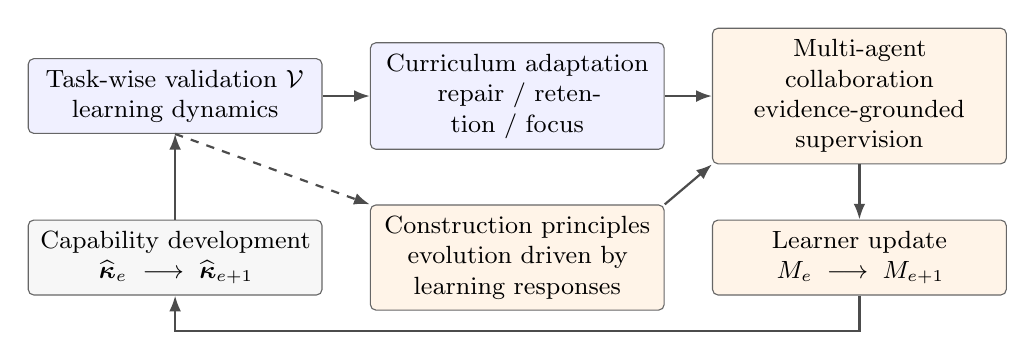
\begin{tikzpicture}[
  box/.style={draw=black!60,rounded corners=2pt,align=center,font=\small,
    minimum height=0.80cm,text width=3.45cm,inner sep=4pt},
  arrow/.style={-{Latex[length=2mm]},thick,draw=black!70},
  feed/.style={arrow,dashed},node distance=0.7cm and 0.6cm]
  \node[box,fill=blue!6] (feedback) {\FigFeedback};
  \node[box,fill=blue!6,right=of feedback] (policy) {\FigPolicy};
  \node[box,fill=orange!9,right=of policy] (synth) {\FigSynthesis};
  \node[box,fill=orange!9,below=of synth] (student) {\FigStudent};
  \node[box,fill=orange!9,left=of student] (strategy) {\FigStrategy};
  \node[box,fill=black!3,left=of strategy] (record) {\FigRecord};
  \draw[arrow] (feedback) -- (policy);
  \draw[arrow] (policy) -- (synth);
  \draw[arrow] (synth) -- (student);
  \draw[arrow] (student.south) -- ++(0,-0.45) -| (record.south);
  \draw[arrow] (record) -- (feedback);
  \draw[feed] (feedback.south) -- (strategy.north west);
  \draw[arrow] (strategy.north east) -- (synth.south west);
\end{tikzpicture}%
}

% An honest placeholder for future measurements, not an illustrative result curve.
\newcommand{\trajectoryplaceholder}{%
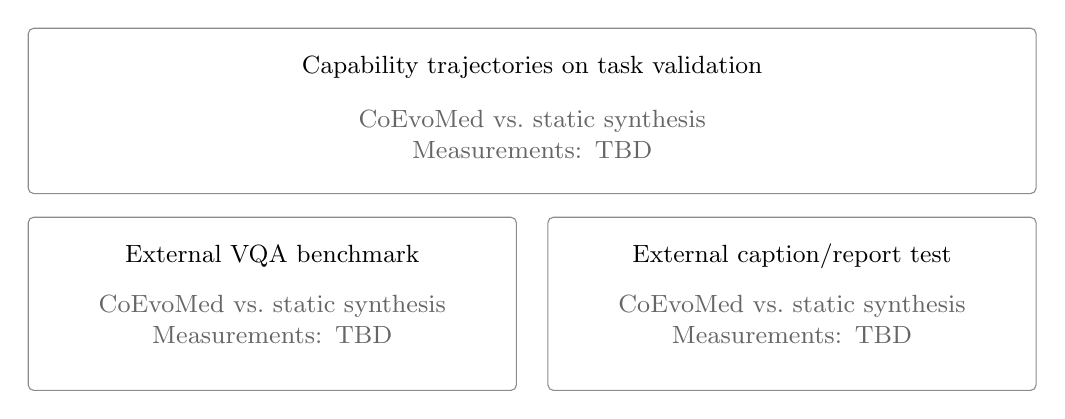
\begin{tikzpicture}[font=\small]
  \draw[draw=black!45,rounded corners=2pt] (0,2.5) rectangle (12.8,4.6);
  \node at (6.4,4.1) {\FigCapability};
  \node[align=center,text width=11.5cm,text=black!60] at (6.4,3.25) {\FigPending};
  \draw[draw=black!45,rounded corners=2pt] (0,0) rectangle (6.2,2.2);
  \draw[draw=black!45,rounded corners=2pt] (6.6,0) rectangle (12.8,2.2);
  \node at (3.1,1.7) {\FigVQA};
  \node at (9.7,1.7) {\FigReport};
  \node[align=center,text width=5.5cm,text=black!60] at (3.1,0.9) {\FigPending};
  \node[align=center,text width=5.5cm,text=black!60] at (9.7,0.9) {\FigPending};
\end{tikzpicture}%
}

\title{\textls[-16]{CoEvoMed: Co-Evolving Supervision Principles}\\and Medical Vision--Language Models}
\hypersetup{pdftitle={CoEvoMed: Co-Evolving Supervision Principles and Medical Vision–Language Models}}
\author{Anonymous Authors}
% Leave \iclrfinalcopy disabled for anonymous review.
\newcommand{\FigFeedback}{Task-wise validation $\mathcal V$\\learning dynamics}
\newcommand{\FigPolicy}{Curriculum adaptation\\repair / retention / focus}
\newcommand{\FigSynthesis}{Multi-agent collaboration\\evidence-grounded supervision}
\newcommand{\FigStudent}{Learner update\\$M_e\longrightarrow M_{e+1}$}
\newcommand{\FigStrategy}{Construction principles\\evolution driven by learning responses}
\newcommand{\FigRecord}{Capability development\\$\widehat{\boldsymbol\kappa}_e\longrightarrow\widehat{\boldsymbol\kappa}_{e+1}$}
\newcommand{\FigExternal}{External testing\\$\mathcal B_{\mathrm{ext}}$ (after run)}
\newcommand{\FigVQA}{External VQA benchmark}
\newcommand{\FigReport}{External caption/report test}
\newcommand{\FigPending}{CoEvoMed vs.\ static synthesis\\Measurements: TBD}
\newcommand{\FigCapability}{Capability trajectories on task validation}
\begin{document}
\maketitle
\begin{abstract}
\frenchspacing
Training medical vision--language models requires supervision that adapts as the learner's capabilities change across tasks. Existing pipelines typically rely on repeated manual error analysis and task-specific training data construction, making this adaptation costly. We introduce CoEvoMed, a co-evolutionary framework that couples a medical vision--language learner with a multi-agent supervision process integrating the evolution of construction principles with curriculum allocation. These reusable principles define question intent, guide how responses draw on medical evidence, and clarify conceptual distinctions in training examples. A revision agent updates these principles in response to the learner's evolving task-specific capabilities, guided by comparisons of factual consistency and task alignment between examples generated from the same medical evidence. Under fixed budgets for each task, curriculum allocation adjusts construction effort according to the learner's capability profile and learning progress. Using CoEvoMed, we train an 8B model supporting both 2D and 3D medical tasks. It surpasses Hulu-Med-7B by 1.15--4.80 percentage points on four 2D VQA benchmarks and achieves higher RaTEScore on MIMIC-CXR and IU-Xray, while delivering strong performance on 3D recognition, question answering, and report generation. Results at 32B further support the scalability of the framework.
\end{abstract}
\begingroup
\setlength{\intextsep}{3pt}
\begin{figure}[H]
\centering
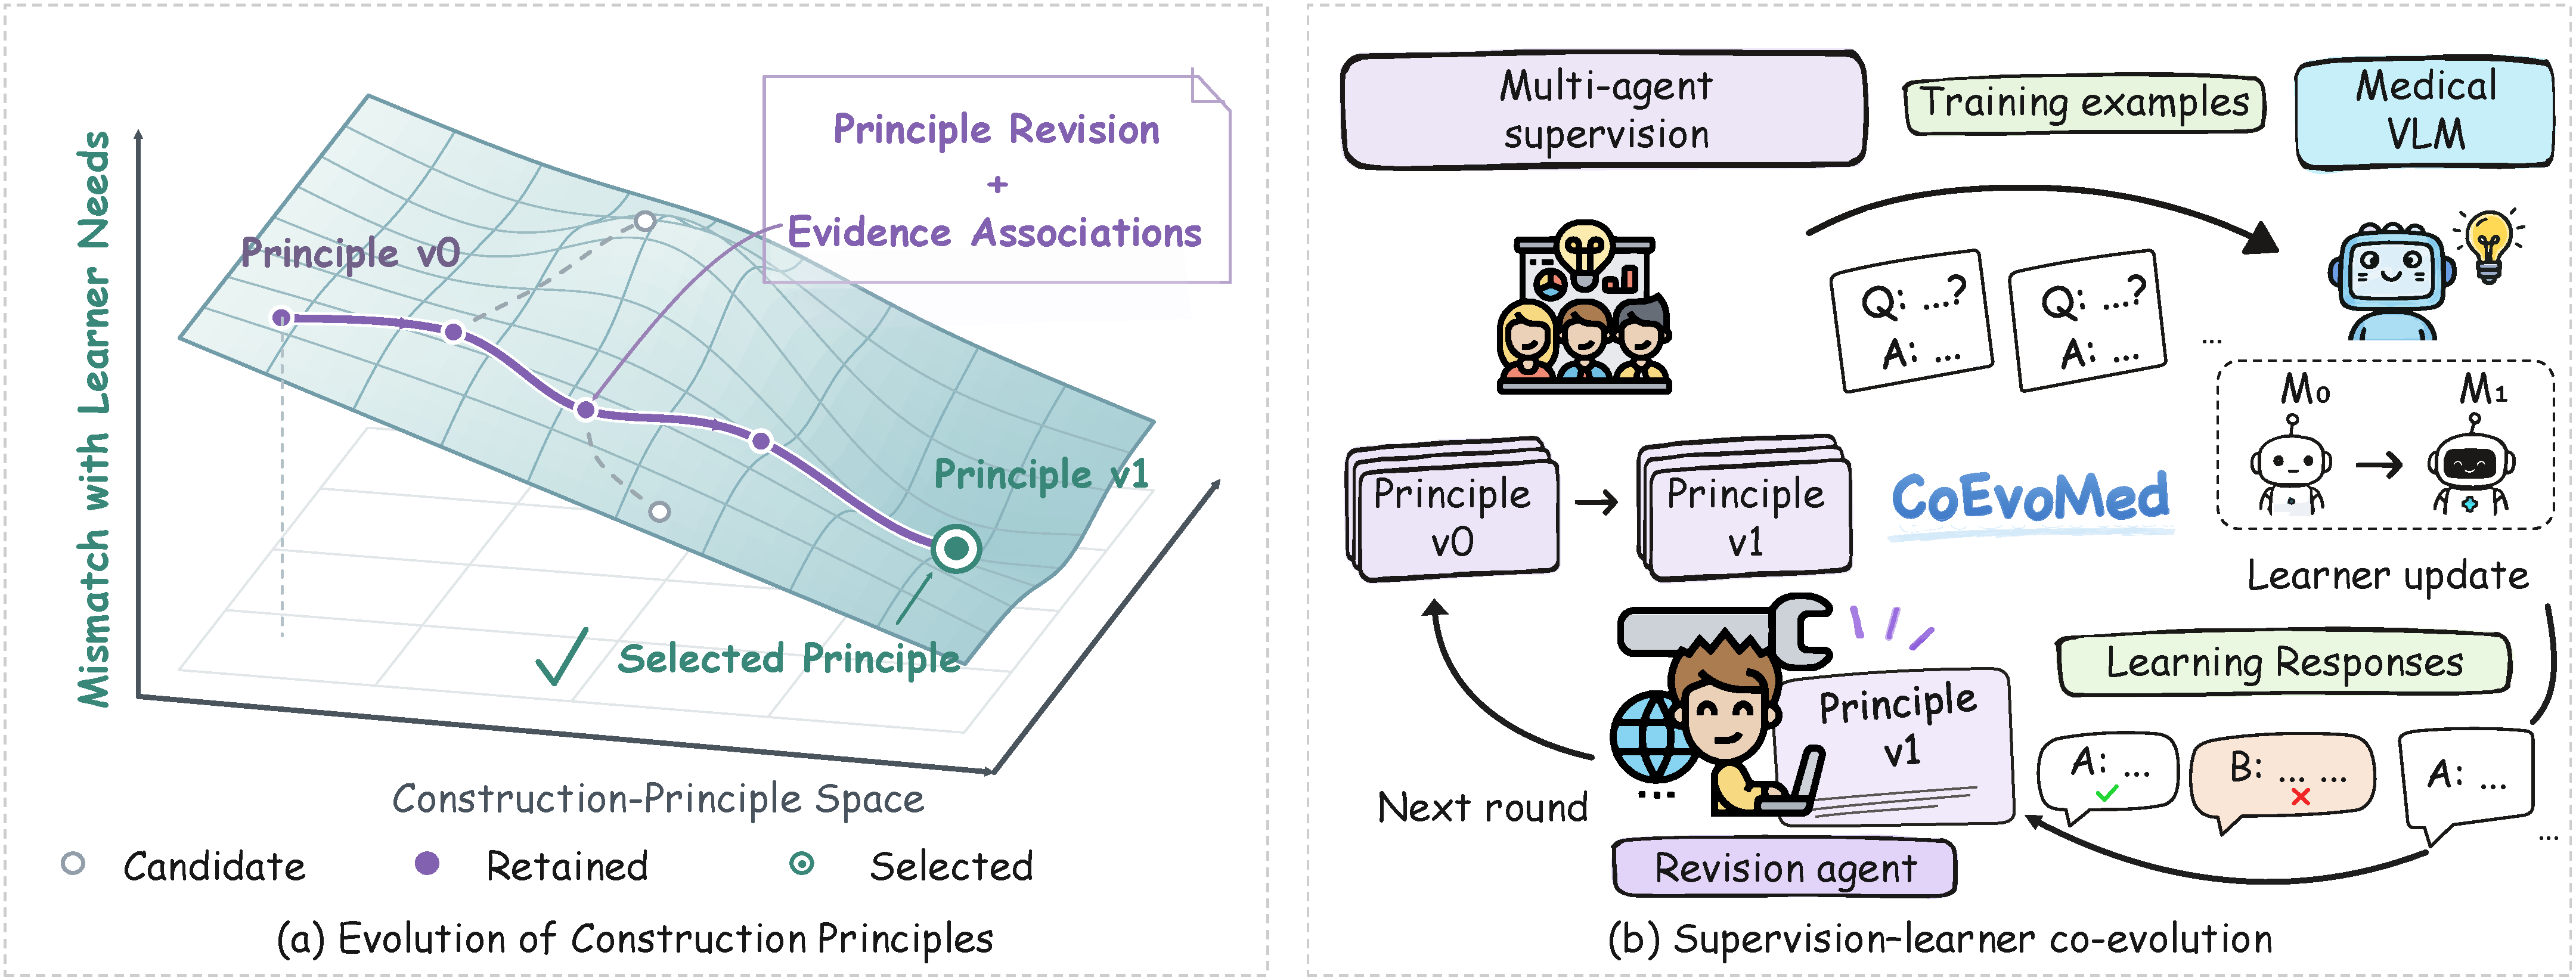
\includegraphics[width=\linewidth]{figures/evoforma_concept.pdf}
\caption{Co-evolution in CoEvoMed. (a) Learning responses guide principle evolution. (b) The multi-agent process connects supervision construction, learner updates, and principle revision.}
\label{fig:concept}
\end{figure}
\endgroup
\vspace{-7pt}
\FloatBarrier
\section{Introduction}
\label{sec:intro}

The knowledge covered by training data and the organization of its supervision constrain capability formation in medical multimodal models. The former defines the medical evidence available for learning; the latter organizes the task objectives and reasoning relations to be learned from that evidence. Supervisory utility depends on alignment with the learner's current state. As training proceeds, task-specific mastery and learning gains evolve unevenly, limiting the continued suitability of a fixed organization of training supervision. This motivates treating data construction as an endogenous component of training, with supervision construction and training allocation continually adapting to learner development.

Existing data refinement practices often rely on manual error inspection and failure mode analysis~\citep{wu2019errudite}, followed by targeted supervision construction~\citep{khan2025dataenvgym}. Repeated fine-grained diagnosis and supervision design incur substantial human effort~\citep{ribeiro2022adaptive} and limit the timely translation of evolving learning needs into systematic training interventions. This limitation motivates a shift from static supervision provision to supervision construction driven by learning responses: observed learning responses inform revisions to reusable construction principles, while realized learning gains regulate the allocation of training resources, establishing a reciprocal evolutionary process between supervision construction and model learning.

Curriculum learning adapts content selection and allocation~\citep{bengio2009curriculum,matiisen2017teacher}; DataEnvGym uses student feedback for iterative data generation~\citep{khan2025dataenvgym}; Evo-PI evolves principles for evaluating and rewarding medical reasoning~\citep{zheng2026evopi}. We focus on the reciprocal development of construction principles and learner capabilities: learning responses revise how evidence is expressed as supervision, and those revisions shape subsequent learning. This connects the evolution of supervision construction with the allocation of finite construction resources.

We introduce \emph{CoEvoMed}, a framework for co-evolving supervision agents and multimodal learners through \emph{supervision construction driven by learning responses}. CoEvoMed constructs training supervision from medical evidence through reusable principles. The learner updates its parameters using this supervision, while task-specific assessments of its capability profile guide the evolution of the principles and the adaptation of subsequent supervision. Residual errors guide their revision, while realized learning gains regulate construction effort across capabilities under a fixed budget. Multi-agent collaboration compares candidate principles under matched evidence and objectives, evaluating supervisory alignment and factual consistency. Selected principles shape subsequent supervision; the learner's ensuing responses guide further revision. Independent validation sets organized by task supply these responses, a shared support set grounds construction in medical evidence, and independent external benchmarks measure outcomes. The evolution of construction principles and the development of learner capabilities jointly shape the learning trajectory.

\begingroup
\frenchspacing
Overall, our main contributions are summarized as follows:

\noindent\textbullet\enspace We propose a co-evolutionary framework that incorporates the evolution of construction principles into learner training, coupling supervision construction and capability development through reciprocal feedback.

\noindent\textbullet\enspace We develop a curriculum allocation policy that balances the development of weaker capabilities with the retention of acquired capabilities. Learning progress informs how a fixed construction budget is redistributed as the learner develops.

\noindent\textbullet\enspace We design a multi-agent system that integrates curriculum allocation and principle evolution. Allocation directs construction effort across capabilities, while evolving principles guide how medical evidence is organized into training examples.
\par\endgroup


\section{Related Work}
\label{sec:related}

\subsection{Curriculum Learning and Adaptive Supervision}

Curriculum learning orders examples by difficulty~\citep{bengio2009curriculum}; adaptive teaching selects them according to learning progress or learner state~\citep{matiisen2017teacher,liu2017iterative}. Beyond selection, Generative Teaching Networks optimize synthetic supervision through meta-gradients~\citep{such2020generative}, and DataEnvGym guides data generation with learner feedback~\citep{khan2025dataenvgym}. Recent approaches couple task generation, visual supervision, or task knowledge with learner development~\citep{huang2026rzero,zhang2026viper,wu2026k2}. CoEvoMed jointly adapts supervision construction and curriculum allocation: reusable construction principles evolve with learning responses, while realized gains guide construction effort across capabilities.

\subsection{Multi-agent adaptation and co-evolution}

Self-Instruct generates instruction-following supervision~\citep{wang2023self}. AutoGen organizes agent conversations~\citep{wu2024autogen}, Graph-of-Agents adapts collaboration structures~\citep{yun2026graph}, and Automated Design of Agentic Systems searches agent programs through a meta agent~\citep{hu2025automated}. Feedback supports output refinement in Self-Refine~\citep{madaan2023selfrefine}, cross-trial reflection in Reflexion~\citep{shinn2023reflexion}, context refinement in ACE~\citep{zhang2026agentic}, and policy optimization through interaction rewards in CoMAS~\citep{xue2026comas}. CoEvoMed connects the revision of construction principles with the development of learner capabilities: learning responses revise evidence-grounded construction principles, whose induced supervision shapes subsequent learning.

\subsection{Medical multimodal learning}

Medical vision-language tasks span radiology, pathology, literature-derived VQA, and report generation~\citep{lau2018dataset,liu2021slake,he2020pathvqa,zhang2024pmc,johnson2019mimic,demnerfushman2016preparing}. LLaVA-Med and Med-Flamingo study biomedical instruction tuning and few-shot adaptation~\citep{li2023llava,moor2023med}. RadFM integrates 2D/3D radiological inputs with text~\citep{wu2025radfm}; M3D develops volumetric image--text and instruction data~\citep{bai2024m3d}. MedVLSynther combines source-conditioned generation with rubric-based verification~\citep{huang2026synthesizing}, and MMedAgent-RL introduces specialist-reliability curricula~\citep{xia2026mmedagent}. CoEvoMed studies supervision construction adapted to the learner's capabilities across visual settings and backbone families.

\section{Problem formulation}
\label{sec:problem}

We formalize the co-evolution of construction principles and learner capabilities, with curriculum allocation modeled as a sequential decision problem. At round $e$, capability-specific shares $\boldsymbol q_e$ allocate a finite construction budget across capability cells defined within each task, subject to fixed task-level quotas. Construction principles $\Sigma_e$ are reusable specifications that determine how medical evidence is organized into supervision for a target capability. These principles define question intent, guide how responses draw on medical evidence, and clarify conceptual distinctions.

\subsection{Learner state and curriculum allocation}

At round $e$, the learner $M_e$ is assessed on independent validation sets $\mathcal V=\{\mathcal V_t\}_{t\in\mathcal T}$ for tasks $\mathcal T$. Support set $\mathcal S$ supplies medical visual evidence and associated text for supervision construction; independent external benchmarks evaluate generalization. Predefined capability cells form $\mathcal C$, with each cell $c$ assessed on a fixed nonempty subset $\mathcal V_c\subseteq\mathcal V_t$. A capability evaluation functional $\mathcal J_c$ maps predictive behavior to empirical mastery:
\begin{equation}
\mathcal J_c[M_e]=\frac{1}{|\mathcal V_c|}\sum_{z\in\mathcal V_c}u_c(M_e,z),
\qquad
\widehat{\boldsymbol\kappa}_e=\bigl(\mathcal J_c[M_e]\bigr)_{c\in\mathcal C}.
\label{eq:capability_level}
\end{equation}
Here $u_c$ is a fixed evaluation rule that assigns a score to each example, with higher scores indicating better performance. The vector $\widehat{\boldsymbol\kappa}_e$ is the observable capability profile. Task performance and error evidence constitute observation $o_e$.

The curriculum planner selects action $a_e$ from history summary $\mathbf{s}_e=\Phi(h_e)$, where $h_e$ records observations, actions, and rewards through round $e$. We model this interaction as a finite-horizon partially observable Markov decision process~\citep{kaelbling1998planning,matiisen2017teacher}. The complete state $X_e$ includes learner parameters and optimization state, active construction principles, revision history, scheduling information, and remaining resources. Under the rule $\mathscr E$ governing principle evolution,
\begin{equation}
P(X_{e+1}\mid X_{0:e},a_{0:e})
=P_{\mathscr E}(X_{e+1}\mid X_e,a_e).
\label{eq:transition}
\end{equation}
The transition comprises supervision construction, verification, learner updates, and principle revision driven by learning responses. Appendix~\ref{app:formalization} specifies the state and observation model.

% Queue the full-width framework for the next page top before the method section.
\begin{figure}[!t]
\centering
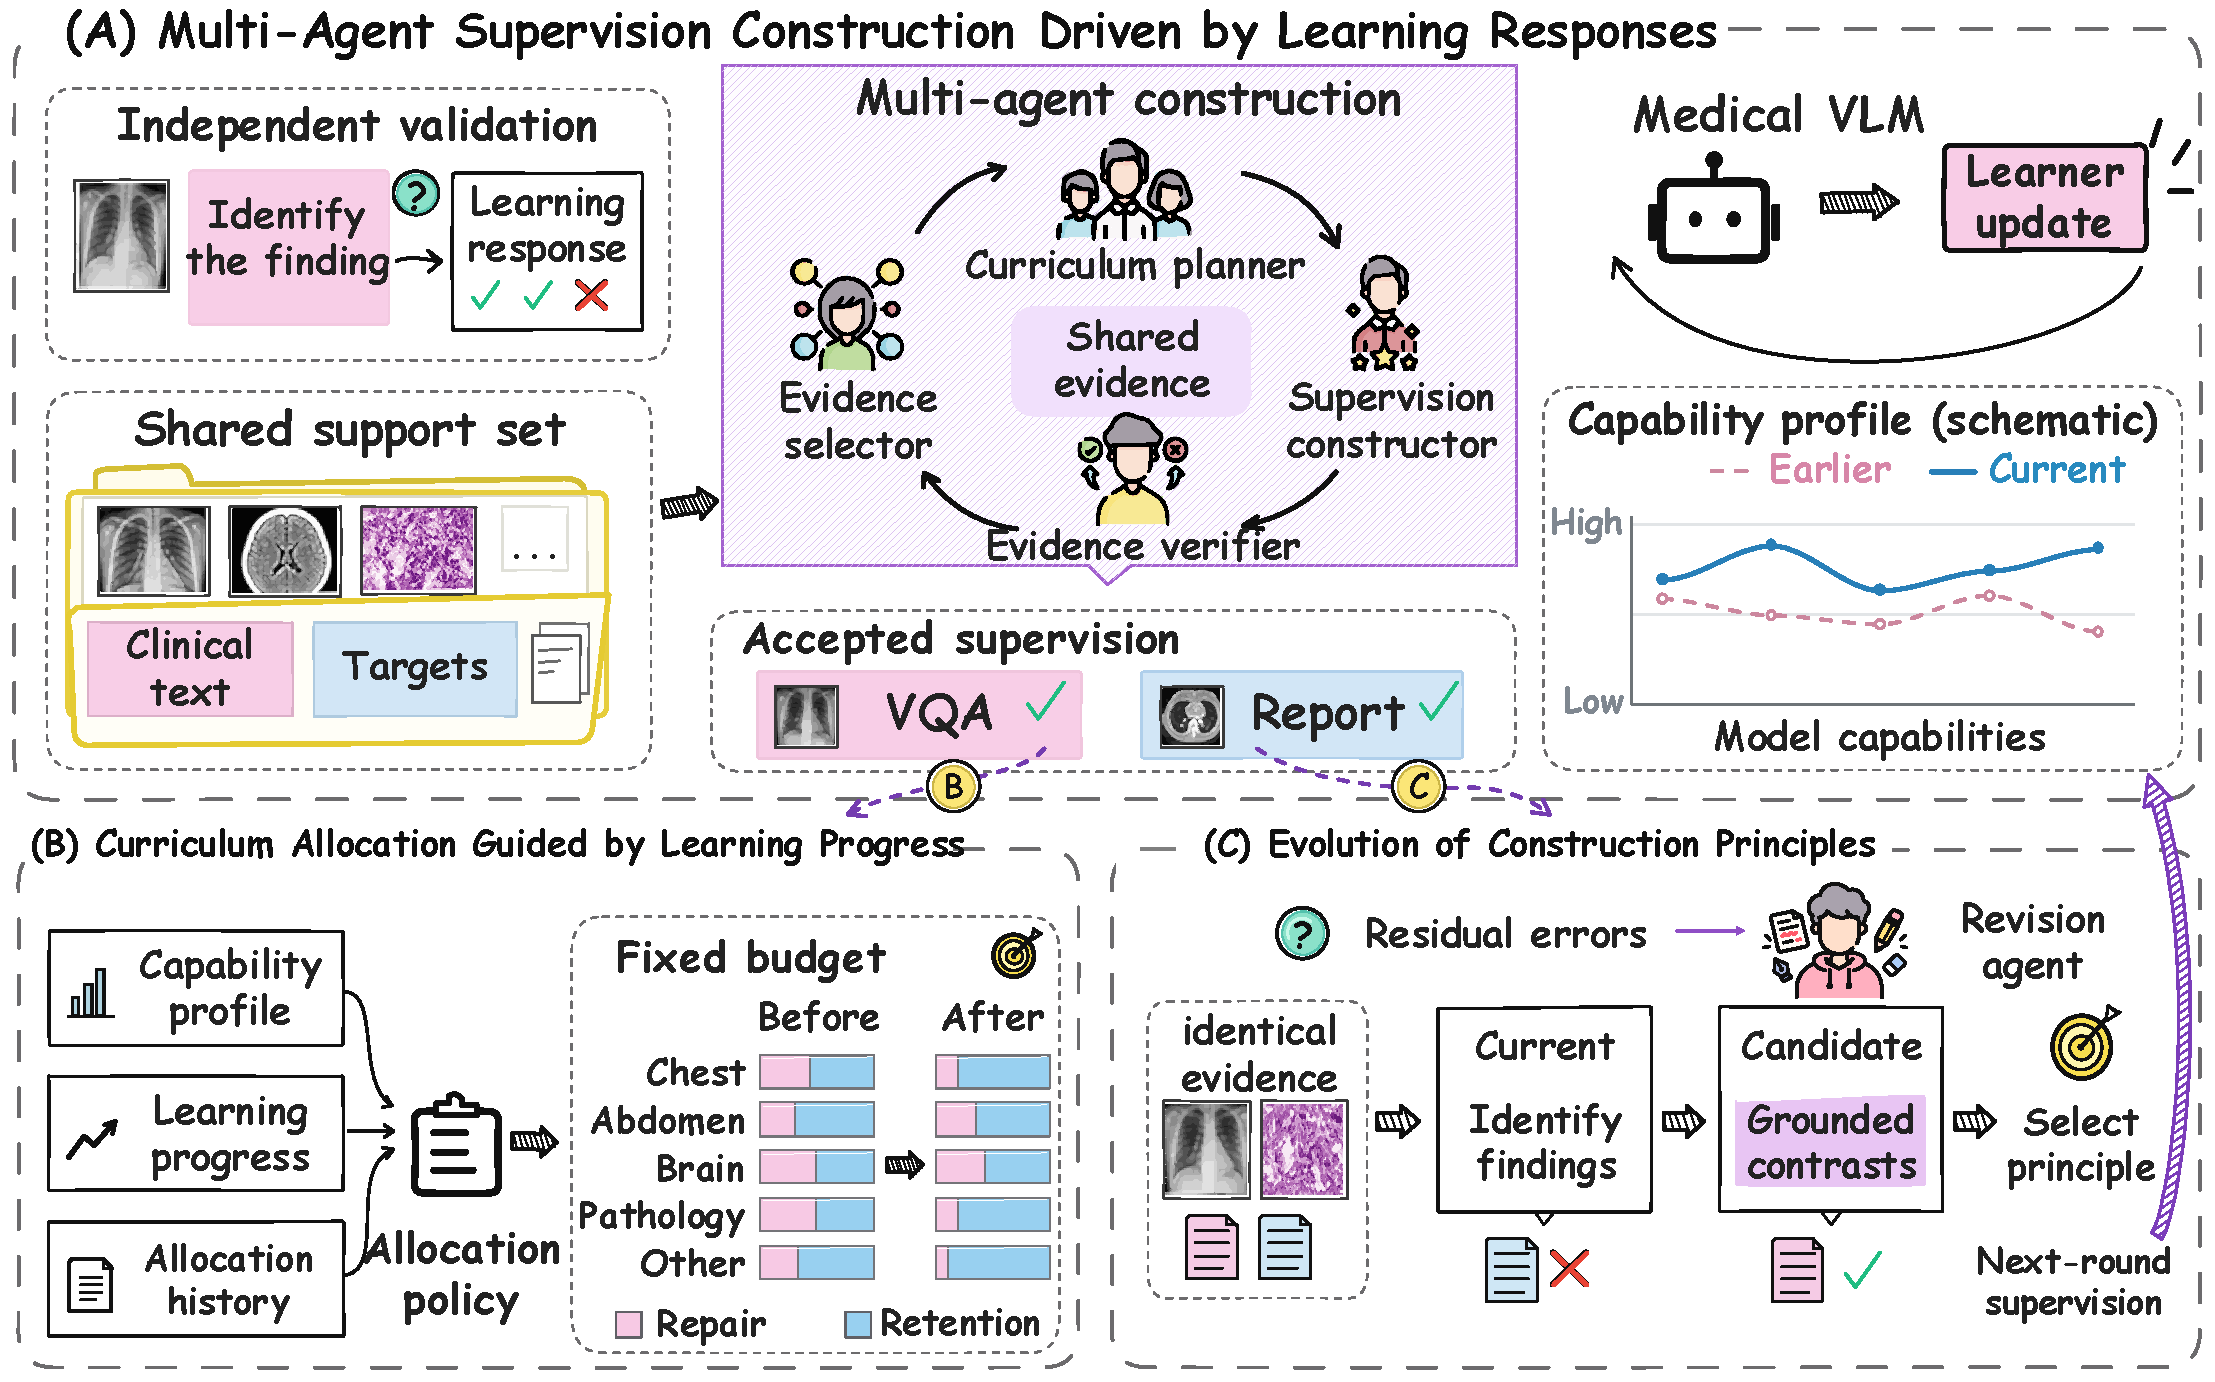
\includegraphics[width=\linewidth]{figures/evoforma_framework.pdf}
\caption{CoEvoMed framework. (A) Multi-agent collaboration constructs and verifies supervision from medical evidence; learner updates yield responses on independent task validation sets. (B) Learning progress guides curriculum allocation under fixed task budgets. (C) The revision agent uses learner responses to revise construction principles and compares supervision generated by current and candidate principles from the same evidence; accepted revisions guide subsequent construction.}
\label{fig:framework}
\end{figure}


\subsection{Supervision construction}
\label{sec:supervision_evolution}

Candidate training examples $z=(v,x,y)$ comprise a visual input, instruction, and target response, with distribution
\begin{equation}
\widetilde p_e(z)=\sum_{c\in\mathcal C}q_{e,c}\,
g_{e,c}(z;\Sigma_e,\mathcal S).
\label{eq:supervision_mixture}
\end{equation}
Here $g_{e,c}$ denotes the probability distribution over candidate training examples for capability cell $c$ at round $e$, induced by evidence selection and supervision construction under $\Sigma_e$ using $\mathcal S$, before verification. Nonnegative shares $q_{e,c}$ sum to one. Principle evolution changes the component content, while allocation changes its relative investment. Evidence-grounded verification yields accepted supervision $\mathcal D_e^{\mathrm{syn}}$; subsequent mixing determines training exposure.

\subsection{Learner updates and policy objective}

The training mixture $\mathcal D_e^{\mathrm{mix}}$ combines accepted supervision $\mathcal D_e^{\mathrm{syn}}$ with permitted original or replay data $\mathcal R_e$ reserved for training. The learner update is
\begin{equation}
M_{e+1}=\mathcal U(M_e,\mathcal D_e^{\mathrm{mix}}),
\label{eq:learning_dynamics}
\end{equation}
where $\mathcal U$ follows the prescribed training procedure and optimization state. Successive capability profiles track the learner's development over $E$ rounds. Responses from $M_{e+1}$ enter $h_{e+1}$ and revise $\Sigma_{e+1}$ through Equation~\ref{eq:strategy_evolution}, linking principle evolution to subsequent learning.

Within these dynamics, the allocation policy maximizes cumulative validation progress:
\begin{equation}
\max_{\pi\in\Pi_{\mathrm{adm}}}
\E_{\pi}\left[\sum_{e=0}^{E-1}\gamma^e r_e\right],
\label{eq:objective}
\end{equation}
where $\Pi_{\mathrm{adm}}$ contains policies satisfying the construction budget and task quotas, and $\gamma\in[0,1]$ is the discount factor. The reward $r_e$ weights validation gains for VQA and report generation equally (Section~\ref{sec:curriculum}). Appendix~\ref{app:cumulative_gains} relates cumulative gains to performance across rounds.

\FloatBarrier

\section{CoEvoMed: co-evolving supervision agents and multimodal learners}
\label{sec:method}

CoEvoMed couples supervision construction with learner updates through learning responses (Figure~\ref{fig:framework}). Its multi-agent system integrates curriculum allocation and principle evolution: allocation directs construction effort, while revised principles change how the agents organize medical evidence into supervision.

\subsection{Multi-Agent Supervision Construction Driven by Learning Responses}
\label{sec:multiagent}

The curriculum planner translates capability feedback into allocation shares and construction targets. The evidence selector retrieves compatible visual records and supported facts from $\mathcal S$; the supervision constructor applies $\Sigma_e$ to form question--answer pairs or reports, and the evidence verifier checks factual consistency, visual dependence, validity, and duplication. Accepted supervision $\mathcal D_e^{\mathrm{syn}}$ retains evidence and principle provenance for subsequent assessment.

The learner minimizes negative log-likelihood over response tokens in $\mathcal D_e^{\mathrm{mix}}$ under the prescribed budget (Appendix~\ref{app:learner_objective}). After each update, CoEvoMed aligns successive predictions on the same task-validation cases. The observed increment for cell $c$ is
\begin{equation}
\widehat{\Delta\kappa}_e(c)=\mathcal J_c[M_e]-\mathcal J_c[M_{e-1}],
\quad e\geq1.
\label{eq:capability_change}
\end{equation}
Paired changes distinguish resolved deficiencies, regressions in acquired capabilities, and persistent gaps, identifying repair and retention needs beyond net progress. The summary $\mathbf{s}_e$ combines current mastery, these changes, and allocation history to guide curriculum allocation. Residual errors in the learner's responses reveal task-specific gaps between current capabilities and task demands; their semantics guide construction targets and principle revision.

An evolution window groups training rounds for assessing principle usage and learning responses. At each window's end, the revision agent proposes candidates from residual errors. Comparisons under matched evidence determine which revisions guide subsequent supervision construction (Section~\ref{sec:strategy_evolution}). The complete procedure appears in Appendix~\ref{app:algorithm}.

\subsection{Curriculum Allocation Guided by Learning Progress}
\label{sec:curriculum}

The curriculum planner uses the curriculum allocation policy to select $a_e\sim\mu_{\theta_e}(\cdot\mid \mathbf{s}_e)$, balancing repair and retention and deciding whether to focus on capabilities with the strongest error evidence. Repair targets unresolved gaps in weaker capabilities and recent regressions; retention maintains coverage of acquired capabilities. The allocation map $\mathcal A$ translates the action and historical evidence into construction shares:
\begin{equation}
\boldsymbol q_e=\mathcal A(a_e,h_e),\qquad
\sum_{c\in\mathcal C_t}q_{e,c}=\bar q_t,
\label{eq:quota}
\end{equation}
where $\mathcal C_t$ contains the cells of task $t$ and $\bar q_t$ is its prescribed share. Thus, adaptation redistributes investment within fixed task budgets. These shares weight candidates in Equation~\ref{eq:supervision_mixture}; verification and mixing determine realized training exposure.

Let $U_t^{\mathrm{val}}$ evaluate the learner on $\mathcal V_t$ and $\delta_{e,t}=U_t^{\mathrm{val}}(M_{e+1})-U_t^{\mathrm{val}}(M_e)$. The reward balances VQA tasks $\mathcal T_{\mathrm V}$ and report tasks $\mathcal T_{\mathrm R}$:
\begin{equation}
r_e=G_e=\frac{1}{2|\mathcal T_{\mathrm V}|}\sum_{t\in\mathcal T_{\mathrm V}}\delta_{e,t}
+\frac{1}{2|\mathcal T_{\mathrm R}|}\sum_{t\in\mathcal T_{\mathrm R}}\delta_{e,t}.
\label{eq:gain}
\end{equation}
Evaluation scales remain fixed, so the signed reward retains gains and regressions. Behavior cloning initializes the curriculum planner. PPO with generalized advantage estimation then optimizes Equation~\ref{eq:objective} through on-policy interactions with the learner~\citep{schulman2017proximal,schulman2016high}. Appendix~\ref{app:implementation} specifies the mixed policy and optimization settings.

% Queue Table 1 early to preserve its page-top placement.
\begin{table}[!t]
\centering\small
\caption{Medical VQA accuracy (\%). Bold marks CoEvoMed; its 8B scores use R7.}
\label{tab:main}
\setlength{\tabcolsep}{4pt}
\renewcommand{\arraystretch}{1.05}
\begin{tabularx}{\linewidth}{@{}Y*{4}{>{\centering\arraybackslash}p{0.14\linewidth}}@{}}
\toprule
Models & PMC-VQA & VQA-RAD & SLAKE & PathVQA\\
\MainResultsRows
\end{tabularx}
\end{table}

\subsection{Evolution of Construction Principles}
\label{sec:strategy_evolution}

Curriculum allocation controls construction effort across capabilities. Construction principles $\Sigma_e$ specify question intent, evidence--response relations, and conceptual distinctions; their suitability depends on the learner's capability state. CoEvoMed revises these reusable principles as learning needs evolve.

At each window's end, sufficiently used principles with nonpositive net repair are considered for revision, where net repair counts repaired cases minus regressed cases. The semantics of residual errors guide principle revision while the target capability and medical facts remain fixed. For example, localization errors motivate more explicit associations between regional evidence and the target response.

Current and candidate principles generate supervision from identical evidence under matched quotas. Selection assesses factual consistency and task alignment, including whether revisions express the targeted evidence associations, conceptual contrasts, or fact coverage. Usable yield (the proportion of evidence assignments producing usable supervision) and paired coverage (the proportion producing usable supervision under both principles) provide screening criteria; Appendix~\ref{app:implementation} specifies their thresholds.

Accepted revisions persist as active construction principles~\citep{zhang2026agentic}. Their supervision shapes learner updates, whose validation responses guide further revision:
\begin{equation}
\Sigma_{e+1}=\mathscr E(\Sigma_e,h_{e+1},\mathcal S).
\label{eq:strategy_evolution}
\end{equation}
Here $h_{e+1}$ includes observations and rewards after the learner update. The operator retains active principles between evolution boundaries and when candidates are rejected.

\section{Experiments}
\label{sec:experiments}

\subsection{Experimental setup}

The 2D suite comprises VQA-RAD, SLAKE, PMC-VQA, and PathVQA~\citep{lau2018dataset,liu2021slake,zhang2024pmc,he2020pathvqa}, plus MIMIC-CXR and IU-Xray report generation~\citep{johnson2019mimic,demnerfushman2016preparing}. 3D evaluation covers closed-ended M3D-VQA, open-ended 3D-RAD, and AMOS-MM reports~\citep{bai2024m3d,gai2025threedrad,ji2024amosmm}. Qwen3-VL-8B-Instruct~\citep{bai2025qwen3} is the primary learner; Gemma-3-4B-IT~\citep{gemmateam2025gemma} and InternVL3-9B~\citep{zhu2025internvl3} test cross-backbone applicability, with InternVL results in Appendix~\ref{app:internvl}. Task validation guides adaptation, support evidence grounds supervision, and external benchmarks measure outcomes. Published baselines include Hulu-Med~\citep{jiang2025hulumed}, Lingshu~\citep{lasateam2025lingshu}, MedVLSynther-7B~\citep{huang2026synthesizing}, and CURE-4B~\citep{messina2026cure}.



\subsection{Medical multimodal performance}

CoEvoMed-8B exceeds Hulu-Med-7B by 1.15--4.80 accuracy points across the four VQA benchmarks, while CoEvoMed-32B leads all compared models on each benchmark (Table~\ref{tab:main}). Report generation reaches 68.22 on IU-Xray at 8B and 64.33 on MIMIC-CXR at 32B (Figure~\ref{fig:report_results}). All six 8B results use R7, selected for the best overall cross-task balance.

From the same Qwen3-VL-8B initialization, CoEvoMed outperforms direct training on approximately 700,000 raw examples across all four VQA benchmarks while using fewer training examples (Appendix~\ref{app:raw_source}). This comparison supports adaptive supervision construction and curriculum allocation as a source of performance gains beyond the volume of raw data.



\begin{figure}[!htb]
\centering
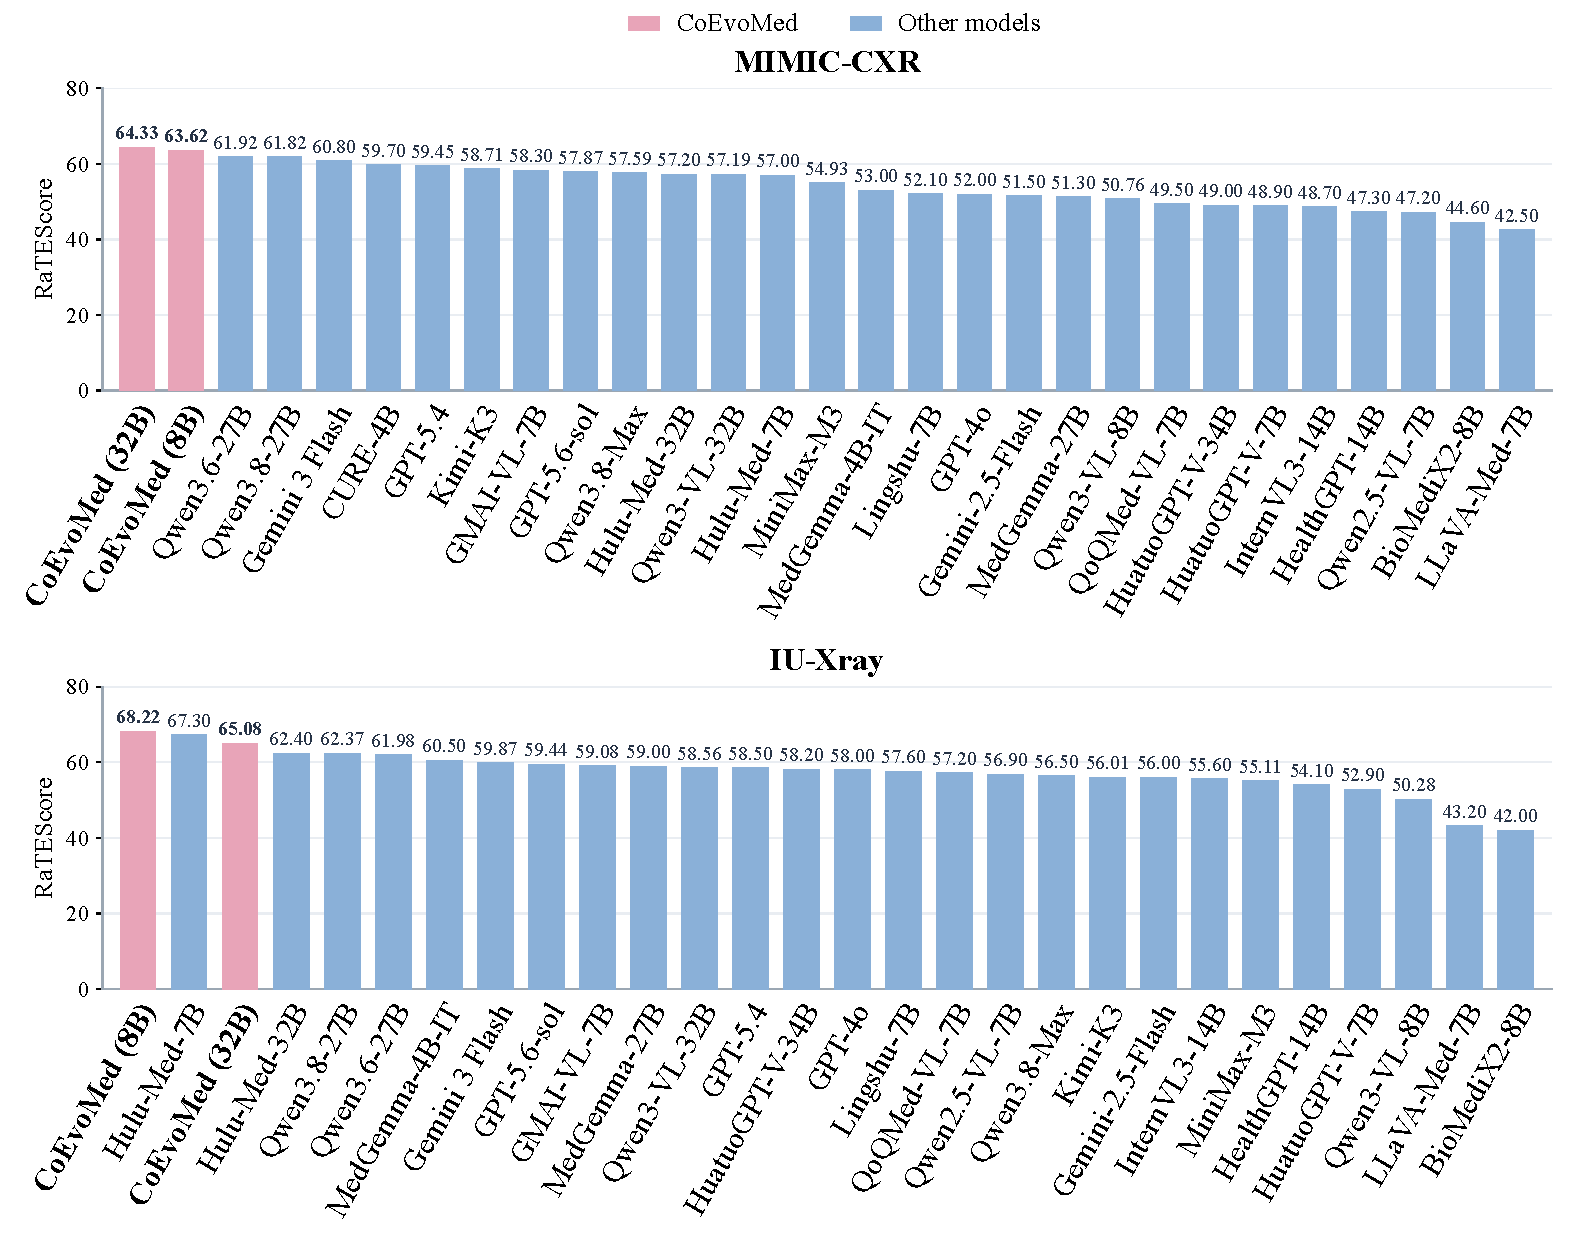
\includegraphics[width=\linewidth,trim=0 14.8bp 0 4bp,clip]{figures/report_ratescore.pdf}
\caption{Report generation on MIMIC-CXR (top, 29 models) and IU-Xray (bottom, 28 models), ranked separately by RaTEScore ($\times100$). Pink denotes CoEvoMed; blue denotes baselines. CURE-4B uses AGRG-29 + GRG. Supplementary metrics appear in Figure~\ref{fig:report_lexical}.}
\label{fig:report_results}
\end{figure}

\paragraph{Applicability to volumetric data.}
CoEvoMed ranks first in the three benchmark summaries in Figure~\ref{fig:3d_main}: M3D-VQA macro accuracy, 3D-RAD macro ROUGE-1, and AMOS-MM RaTEScore. These results extend the evaluation to volumetric question answering and report generation. Category-level results, supplementary metrics, and evaluation details appear in Appendix~\ref{app:3d}.

\begin{figure}[!htb]
\centering
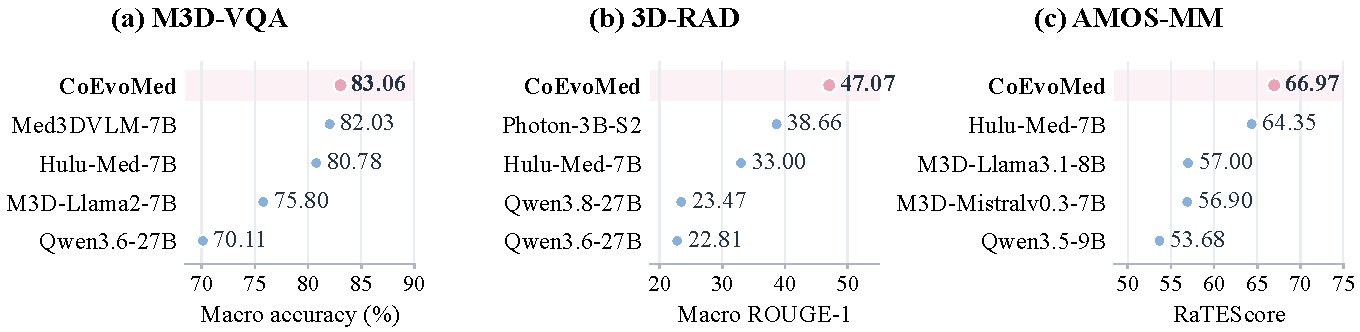
\includegraphics[width=\linewidth]{figures/three_d_main.pdf}
\caption{Volumetric evaluation: (a) M3D-VQA macro accuracy; (b) 3D-RAD macro ROUGE-1; (c) AMOS-MM RaTEScore. Scores are scaled to 100. Each panel shows CoEvoMed (pink) and the four highest-scoring baselines (blue) for its metric within the comparison set in Appendix~\ref{app:3d}.}
\label{fig:3d_main}
\end{figure}

\subsection{Learning dynamics and mechanism analysis}
\label{sec:analysis}
\label{sec:mechanisms}

We examine learning trajectories, feedback--learner alignment, and stage-dependent principle utility. Mechanism comparisons use VQA-RAD and MIMIC-CXR; full results and experimental details appear in Appendix~\ref{app:mechanisms}.

\paragraph{Feedback--learner alignment.}
From the same R5 checkpoint, we jointly vary numerical capability statistics and summaries of error semantics using R2, R3, or R5 validation feedback. Current feedback improves VQA-RAD accuracy by 2.62 percentage points and MIMIC-CXR RaTEScore by 2.77 points, outperforming historical feedback (Table~\ref{tab:ablations}, panel A). This supports aligning curriculum allocation and supervision construction with current capabilities and error patterns.

\paragraph{Dependence on training stage.}
Original and evolved principles show stage-dependent utility at checkpoints after rounds 2 and 5 (R2 and R5) (Table~\ref{tab:ablations}, panel B). On VQA-RAD, original principles lead by 4.22 points at R2, whereas evolved principles lead by 8.26 at R5. On MIMIC-CXR, their difference grows from 0.12 to 9.21 points in favor of evolved principles. This stage dependence supports revising supervision as the learner develops; all six benchmarks appear in Appendix~\ref{app:stage_transfer}.

\begin{table}[H]
\centering\small
\caption{Mechanism ablations: (A) the same R5 learner with R2, R3, or current R5 feedback; (B) original versus evolved construction principles at R2 and R5. VQA-RAD reports accuracy (\%); MIMIC-CXR reports RaTEScore ($\times100$). Reference scores are measured before further training.}
\label{tab:ablations}
\setlength{\tabcolsep}{3.5pt}
\renewcommand{\arraystretch}{1.0}
\begin{minipage}[t]{0.47\linewidth}
\vspace{0pt}
\begin{tabularx}{\linewidth}{Yrr}
\toprule
\multicolumn{3}{l}{\textbf{A. Feedback source at R5}}\\
\midrule
Setting & VQA-RAD & MIMIC-CXR\\
\midrule
R5: Reference & 73.61 & 59.00\\
R2 feedback & 72.51 & 59.11\\
R3 feedback & 71.84 & 58.16\\
\rowcolor{mainOurs} \textbf{R5 feedback} & 76.23 & 61.77\\
\bottomrule
\end{tabularx}
\end{minipage}\hfill
\begin{minipage}[t]{0.50\linewidth}
\vspace{0pt}
\begin{tabularx}{\linewidth}{Yrr}
\toprule
\multicolumn{3}{l}{\textbf{B. Dependence on training stage}}\\
\midrule
Setting & VQA-RAD & MIMIC-CXR\\
\midrule
R2: Reference & 61.64 & 53.31\\
R2: Original & 63.42 & 56.35\\
R2: Evolved & 59.20 & 56.47\\
\midrule
R5: Reference & 73.61 & 59.00\\
R5: Original & 67.97 & 52.56\\
\rowcolor{mainOurs} \textbf{R5: Evolved} & 76.23 & 61.77\\
\bottomrule
\end{tabularx}
\end{minipage}
\end{table}

\paragraph{Cross-backbone applicability.}

On Gemma-3-4B-IT, R7 attains 70.73\% semantic VQA accuracy and 65.89 MIMIC-CXR RaTEScore, improving over Base by 22.39 and 16.23 points (Figure~\ref{fig:gemma_trajectory}). The same checkpoint ties for the highest observed VQA accuracy and achieves the highest report score, supporting applicability beyond Qwen at a smaller model scale. 

\begin{figure}[H]
\centering
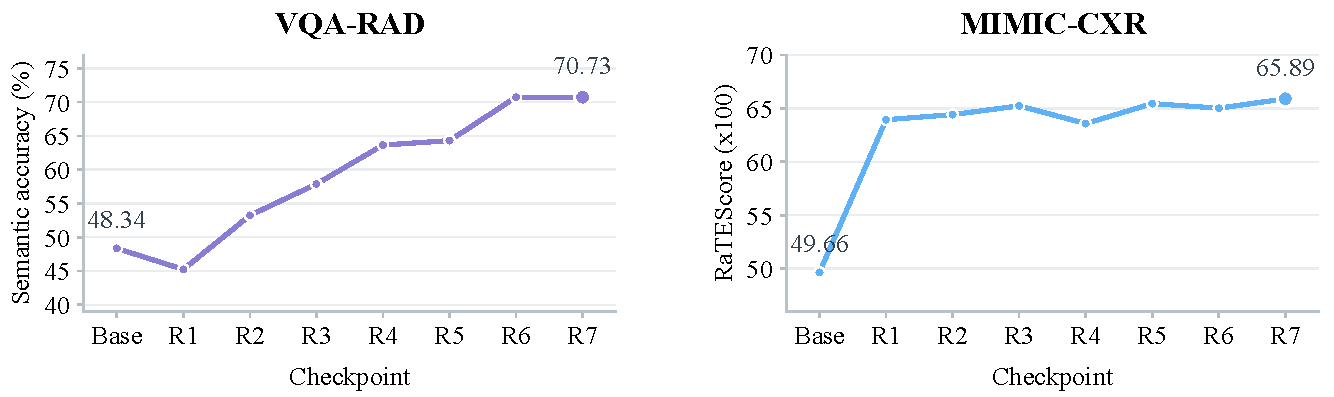
\includegraphics[width=0.85\linewidth]{figures/gemma_trajectory.pdf}
\caption{Cross-backbone evaluation on Gemma-3-4B-IT from Base through R7. VQA-RAD uses semantic accuracy (\%); MIMIC-CXR uses RaTEScore scaled by 100. Both R7 scores belong to the same checkpoint.}
\label{fig:gemma_trajectory}
\end{figure}
\vspace{-10pt}
\begin{figure}[H]
\noindent\begin{minipage}[t]{0.40\textwidth}
\vspace{0pt}
\textbf{Learning trajectories.} Figure~\ref{fig:task_qa} shows that attribute queries improve, organ recognition stabilizes, and localization recovers after declining over R1--R6. These divergent trajectories indicate that capability development is not uniform across tasks, providing the state information used for principle revision and construction allocation. Figure~\ref{fig:trajectory} shows gains on SLAKE, PathVQA, and IU-Xray, peaking at R7--R8. Their agreement with the task-level profiles connects learner responses to externally measured benchmark performance. Together, the profiles characterize capability development and performance on independent external benchmarks.
\end{minipage}\hfill
\begin{minipage}[t]{0.56\textwidth}
\vspace{0pt}\centering
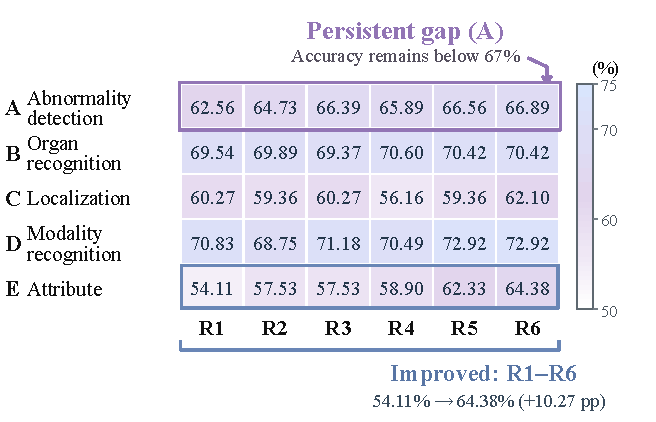
\includegraphics[width=\linewidth]{figures/task_qa_heatmap.pdf}
\caption{Validation accuracy (\%) of the Qwen3-VL-8B learner across five selected QA task categories after completed training rounds R1--R6.}
\label{fig:task_qa}
\end{minipage}
\end{figure}
\vspace{-10pt}
\begin{figure}[H]
\centering
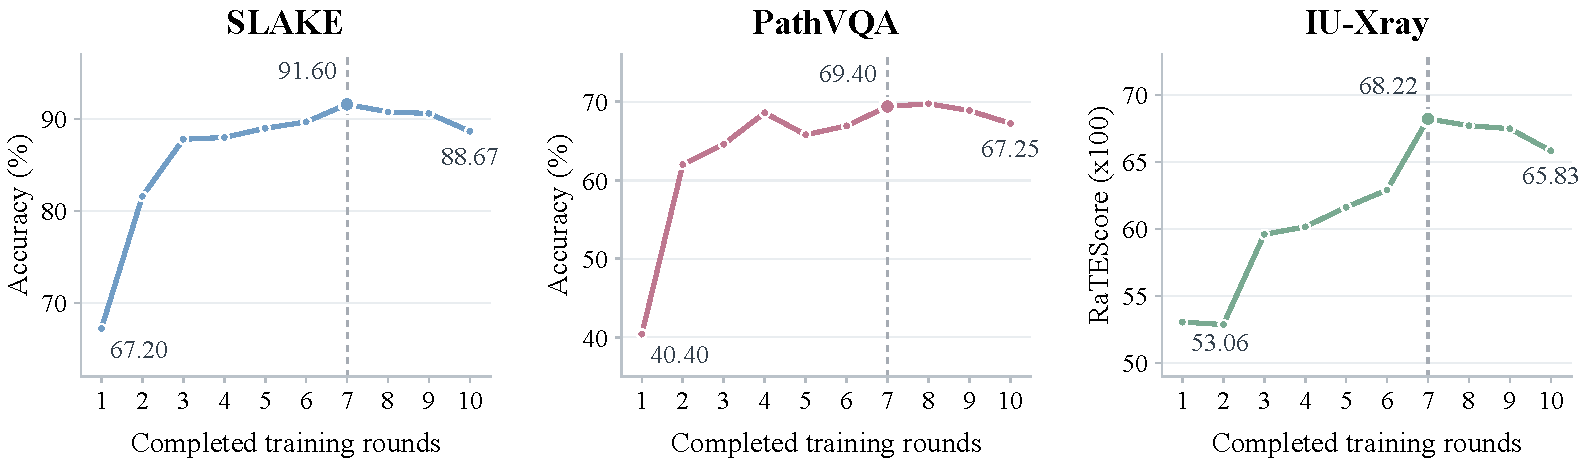
\includegraphics[width=0.85\linewidth]{figures/evolution_trajectory.pdf}
\caption{CoEvoMed-8B trajectories. Dashed lines mark R7, used for all six main 2D results.}
\label{fig:trajectory}
\end{figure}
\vspace{-12pt}
\section{Conclusion}
\label{sec:conclusion}

CoEvoMed treats supervision construction as an evolving component of medical vision--language learning. Construction principles develop in response to the learner's task-specific capabilities, while the resulting supervision shapes subsequent capability development. Curriculum allocation complements this process by distributing a fixed construction budget according to observed learning progress. Multi-agent collaboration connects these two forms of adaptation, using medical evidence to produce supervision whose content and allocation evolve together.

Experiments across 2D VQA, report generation, 3D tasks, and different backbones support the effectiveness of this framework. Comparisons across feedback sources and training stages further show the value of matching supervision construction to the learner's current capability profile. These findings support joint adaptation of how supervision is constructed and where construction effort is allocated as a basis for improving medical multimodal learning.

\label{maintext:end}
\clearpage
\subsection*{AI use statement}
We used AI tools to assist with manuscript writing and language editing. We reviewed the text and take responsibility for the final manuscript.

\subsection*{Ethics statement}
This methodological study uses existing publicly available or authorized research datasets, without new patient recruitment or clinical intervention. Relevant risks include unsupported medical statements, annotation-error propagation, and amplification of source-data or model biases. CoEvoMed incorporates evidence-grounded construction and verification to address factual inconsistency in synthesized supervision. Data access and redistribution of derived material remain subject to the original datasets' licenses, access conditions, and privacy requirements. Clinical deployment would require independent validation, assessment across patient populations, and qualified clinical oversight.

\subsection*{Reproducibility statement}
Sections~\ref{sec:problem}--\ref{sec:method} specify the formulation and mechanisms; Appendix~\ref{app:algorithm} provides training pseudocode. Appendix~\ref{app:implementation} documents learner training settings, curriculum-planner initialization, PPO hyperparameters, supervision budgets and composition, principle-acceptance criteria, agent models, and hardware. Appendix~\ref{app:evaluation} describes 2D and volumetric evaluation splits and inputs, dataset sources and links, evidence preparation, task-validation construction, metrics, checkpoint selection, and feedback--evaluation separation. Appendix~\ref{app:mechanisms} gives ablation settings and full results, and Appendix~\ref{app:formalization} provides formal definitions and the cumulative-gain derivation.

\bibliography{iclr2027_conference}
\bibliographystyle{iclr2027_conference}
\appendix
\clearpage
\section{Complete training procedure}
\label{app:algorithm}

Algorithm~\ref{alg:coevomed} summarizes the co-evolution loop. Here $\pi_\theta$ is the Actor softmax distribution and $\mu$ is the executed policy with uniform exploration. Appendix~\ref{app:implementation} specifies budgets, training mixtures, PPO settings, and revision rules.

\begin{algorithm}[H]
\small
\setlength{\tabcolsep}{4pt}
\renewcommand{\arraystretch}{1.08}
\begin{tabularx}{\linewidth}{@{}rY@{}}
\toprule
\multicolumn{2}{@{}p{\linewidth}@{}}{\textbf{Input:} Learner $M_0$, principles $\Sigma_0$, initialized curriculum Actor--Critic, validation sets $\mathcal V$, support evidence $\mathcal S$, and horizon $E$.}\\
\multicolumn{2}{@{}p{\linewidth}@{}}{\textbf{Output:} Learner checkpoints $\mathcal K_E=(M_0,\ldots,M_E)$ and final principles $\Sigma_E$.}\\
\midrule
1 & Evaluate $M_0$ on $\mathcal V$ for $o_0$; initialize $h_0=(o_0)$, $\mathcal K_0=(M_0)$, and usage statistics.\\
2 & \textbf{for} $e=0,\ldots,E-1$ \textbf{do}\\
3 & \hangindent=1em\hangafter=1\quad $\mathbf{s}_e\leftarrow\Phi(h_e)$; $\mu_{\mathrm{old}}\leftarrow0.8\pi_\theta(\cdot\mid\mathbf{s}_e)+0.05$.\\
4 & \hangindent=1em\hangafter=1\quad $a_e\sim\operatorname{Categorical}(\mu_{\mathrm{old}})$; $\ell_e^{\mathrm{old}}\leftarrow\log\mu_{\mathrm{old}}(a_e)$.\\
5 & \hangindent=1em\hangafter=1\quad $\boldsymbol q_e\leftarrow\mathcal A(a_e,h_e)$, preserving task quotas (Eq.~\ref{eq:quota}).\\
6 & \hangindent=1em\hangafter=1\quad Plan repair/retention targets and select supporting facts from $\mathcal S$ under $\boldsymbol q_e$.\\
7 & \hangindent=1em\hangafter=1\quad Construct and verify $\mathcal D_e^{\mathrm{syn}}$ using $\Sigma_e$; record sources and principle versions.\\
8 & \hangindent=1em\hangafter=1\quad $\mathcal D_e^{\mathrm{mix}}\leftarrow\operatorname{Mix}(\mathcal D_e^{\mathrm{syn}},\mathcal R_e)$; $M_{e+1}\leftarrow\mathcal U(M_e,\mathcal D_e^{\mathrm{mix}})$.\\
9 & \hangindent=1em\hangafter=1\quad Evaluate $M_{e+1}$ on the same $\mathcal V$ for $o_{e+1}$ and paired learning responses.\\
10 & \hangindent=1em\hangafter=1\quad $r_e\leftarrow G_e$ (Eq.~\ref{eq:gain}); $\mathcal K_{e+1}\leftarrow(\mathcal K_e,M_{e+1})$.\\
11 & \hangindent=1em\hangafter=1\quad $h_{e+1}\leftarrow(h_e,a_e,r_e,o_{e+1})$; $\mathbf{s}_{e+1}\leftarrow\Phi(h_{e+1})$.\\
12 & \hangindent=1em\hangafter=1\quad Compute one-step advantage and value target from $(\mathbf{s}_e,a_e,r_e,\mathbf{s}_{e+1})$.\\
13 & \hangindent=1em\hangafter=1\quad \textbf{for} $k=1,\ldots,4$ \textbf{do}\\
14 & \hangindent=2em\hangafter=1\qquad $\mu_{\mathrm{new}}\leftarrow0.8\pi_\theta(\cdot\mid\mathbf{s}_e)+0.05$; $\rho_e\leftarrow\exp\!\left(\log\mu_{\mathrm{new}}(a_e)-\ell_e^{\mathrm{old}}\right)$.\\
15 & \hangindent=2em\hangafter=1\qquad Update Actor--Critic with clipped PPO ($\rho_e$), value loss, and entropy $H(\mu_{\mathrm{new}})$.\\
16 & \hangindent=1em\hangafter=1\quad \textbf{end for}\\
17 & \hangindent=1em\hangafter=1\quad Update window statistics by principle version; $\Sigma_{e+1}\leftarrow\Sigma_e$.\\
18 & \hangindent=1em\hangafter=1\quad \textbf{if} an evolution window ends \textbf{then}\\
19 & \hangindent=2em\hangafter=1\qquad Propose revisions from residual errors for eligible principles, preserving the target capability and medical facts.\\
20 & \hangindent=2em\hangafter=1\qquad Construct and verify paired examples under current/candidate principles using $N=100$ identical evidence assignments and matched quotas; obtain usable sets $I_{\mathrm{cur}},I_{\mathrm{cand}}$.\\
21 & \hangindent=2em\hangafter=1\qquad $\Delta_{\mathrm{use}}\leftarrow\dfrac{|I_{\mathrm{cand}}|-|I_{\mathrm{cur}}|}{N}$; $\rho_{\mathrm{pair}}\leftarrow\dfrac{|I_{\mathrm{cand}}\cap I_{\mathrm{cur}}|}{N}$.\\
22 & \hangindent=2em\hangafter=1\qquad If $\rho_{\mathrm{pair}}\geq0.60$, the revision agent semantically reviews up to 30 common usable pairs.\\
23 & \hangindent=2em\hangafter=1\qquad Replace a principle in $\Sigma_{e+1}$ if $|I_{\mathrm{cand}}|/N\geq0.80$, $\Delta_{\mathrm{use}}\geq-0.05$, $\rho_{\mathrm{pair}}\geq0.60$, and semantic review passes.\\
24 & \hangindent=1em\hangafter=1\quad \textbf{end if}\\
25 & \textbf{end for}\\
26 & \textbf{return} $\mathcal K_E,\Sigma_E$.\\
\bottomrule
\end{tabularx}
\caption{CoEvoMed: supervision construction driven by learning responses.}
\label{alg:coevomed}
\end{algorithm}

Eligible principles have sufficient usage and nonpositive net repair within the evolution window. Semantic review requires the revision to be expressed in generated examples, improve alignment with the targeted errors, and preserve evidence support. Accepted revisions govern the next round; rejected or deferred candidates retain the current version. The stored $\ell_e^{\mathrm{old}}$ remains fixed across the four PPO epochs.

Construction uses selected facts rather than direct image access; verification checks candidates using the image. Linking supervision examples to the construction principle versions used to generate them connects principle usage with validation changes in the corresponding capabilities. The training mixture excludes $\mathcal V$ and external benchmarks $\mathcal B_{\mathrm{ext}}$. Saved checkpoints support offline trajectory analysis; all six main 8B results use R7 (Appendix~\ref{app:checkpoint_selection}). External benchmark results do not guide adaptation.

% Keep Appendix B on its existing page.
\clearpage


\section{Training configuration}
\label{app:implementation}

\paragraph{Learner training.}
Qwen3-VL-8B-Instruct is the primary learner, with Qwen3-VL-32B used for the 2D scaling experiments. Each round continues from the preceding learner's parameters, using accepted evidence-grounded supervision $\mathcal D_e^{\mathrm{syn}}$ mixed with the prescribed original or replay data $\mathcal R_e$. Supervised fine-tuning (FullSFT) updates all parameters of the language model and multimodal merger while freezing the vision tower. The 2D training configuration specifies one full epoch per round over $\mathcal D_e^{\mathrm{mix}}$, with training duration determined by the epoch count (\texttt{max\_steps=-1}). We use AdamW~\citep{loshchilov2019decoupled} with $\beta_1=0.9$, $\beta_2=0.999$, $\epsilon=10^{-8}$, and weight decay $0.1$, excluding biases and other exempt parameters. The language model and merger both use a learning rate of $10^{-5}$, with cosine decay and a warmup ratio of $0.03$. Training uses 24 NVIDIA A100 80\,GB GPUs across three nodes, with eight GPUs per node. A batch size of one per GPU and one gradient accumulation step yield an effective global batch size of 24. Computation uses BF16 and DeepSpeed ZeRO-3~\citep{rajbhandari2020zero}, with gradient checkpointing disabled. For volumetric inputs, TF32 is enabled and the pixel count per slice frame is constrained to 65,536--196,608.
\paragraph{Agent roles and models.}
The five agents coordinate supervision construction, curriculum allocation, and principle revision. The evidence selector uses deepseek-v4-flash to select supporting evidence, and the supervision constructor uses the same model to generate training examples under the construction principles. The evidence verifier uses Qwen3.6-27B to assess evidence support and factual consistency. The curriculum planner allocates construction effort based on capability feedback and learning progress: a learned Actor--Critic selects allocation actions, while deepseek-v4-flash specifies construction targets and provides action labels for supervised initialization. The revision agent uses deepseek-v4-flash to propose and assess revisions to construction principles based on learning responses. Qwen3.6-27B also supports factual evidence extraction and annotation of validation sets.

\paragraph{Per-round supervision size and task composition.}
Each training round incorporates 50,000 supervision examples in $\mathcal D_e^{\mathrm{syn}}$ that pass evidence verification, with an approximate $7:3$ ratio of visual question answering (VQA) to report generation (caption) by sample count. Within the VQA subset, multiple-choice, binary, and short-answer questions follow an approximate $92:4:4$ ratio. These two levels specify the composition across task families and the distribution of response formats within VQA, respectively.

\paragraph{Learner training objective.}
\label{app:learner_objective}
For trainable learner parameters $\phi$, the update in Equation~\ref{eq:learning_dynamics} minimizes
\begin{equation}
\mathcal L_e(\phi)=-\E_{(v,x,y)\sim\mathcal D_e^{\mathrm{mix}}}
\sum_{j=1}^{|y|}\log p_\phi(y_j\mid v,x,y_{<j}),
\label{eq:student}
\end{equation}
where $v$, $x$, and $y$ denote visual input, instruction, and target response. Learning responses are measured on fixed validation cases for each task after each update.

\paragraph{Curriculum-planner initialization.}
The curriculum planner maps a 40-dimensional state through a shared two-layer MLP with hidden widths 128 and 64 to a four-action Actor and a scalar Critic. The four actions are balanced, repair-heavy, weakness-focused, and retention-heavy. Baseline evaluation statistics inform the construction of 800 capability states spanning balanced performance, broad deficiencies, localized deficiencies, and capability regression. The teacher deepseek-v4-flash assigns curriculum action labels. A split by state group yields 640 training and 160 validation states. Cross-entropy supervision initializes the shared MLP and Actor; the checkpoint after epoch 5 achieves the best validation performance and is selected. The Critic output head is initialized with zero weights and bias and subsequently learned from real feedback. The 800 states constitute initialization supervision, separate from online learner interactions.

\paragraph{PPO optimization.}
Each curriculum round comprises a decision, supervision construction, learner training, and validation feedback, yielding one environment transition. The Actor--Critic is updated after every round, with four optimization epochs over that round's rollout. With a one-transition rollout, generalized advantage estimation reduces to a one-step temporal-difference estimate. We use Adam~\citep{kingma2015adam} with learning rate $3\times10^{-4}$, discount $\gamma=0.90$, GAE parameter $\lambda=0.95$, clipping threshold $0.20$, value loss coefficient $0.50$, entropy coefficient $0.01$, and gradient norm limit $0.50$. PPO updates the curriculum planner, while external LLM weights remain fixed. When principle evolution is scheduled, planner optimization precedes principle revision.

\paragraph{Sampling and likelihood ratios under the mixed policy.}
Let $\pi_\theta(\cdot\mid s)=\operatorname{softmax}(\operatorname{Actor}_\theta(s))$. The executed allocation policy combines the Actor with uniform exploration over four actions:
\[
\mu_\theta(a\mid s)=0.8\pi_\theta(a\mid s)+0.05.
\]
Actions are sampled from $\mu_{\theta_{\mathrm{old}}}$, and their log probabilities $\ell_e^{\mathrm{old}}=\log\mu_{\theta_{\mathrm{old}}}(a_e\mid \mathbf{s}_e)$ are stored at sampling time. These values remain fixed throughout the four optimization epochs. Each epoch recomputes the probability under the mixed policy for the stored state and action, giving the PPO ratio
\[
\rho_e(\theta)=\exp\!\left(\log\mu_\theta(a_e\mid \mathbf{s}_e)-\ell_e^{\mathrm{old}}\right)
=\frac{\mu_\theta(a_e\mid \mathbf{s}_e)}{\mu_{\theta_{\mathrm{old}}}(a_e\mid \mathbf{s}_e)}.
\]
Entropy regularization also uses $\mu_\theta$. This executed policy instantiates the allocation policy in Equation~\ref{eq:objective}.

\paragraph{Reward based on learning progress.}
Rewards measure validation gains following actual learner updates. VQA uses accuracy; report generation uses $0.5\,\mathrm{ROUGE\mbox{-}L}+0.3\,\mathrm{BLEU\mbox{-}4}+0.2\,\mathrm{METEOR}$. Gains are averaged within each task family, and the VQA and report families receive equal weight, as in Equation~\ref{eq:gain}.

\paragraph{Principle revision and selection.}
Persistent construction principles specify question intent, evidence--response relations, conceptual contrasts, and diversity. Learning responses observed within each window identify sufficiently used principles with nonpositive net repair. The revision agent uses summaries of residual errors to propose candidates while preserving the target capability and medical facts. Current and candidate principles are compared on the same $N>0$ evidence assignments. Let $I_{\mathrm{cur}}$ and $I_{\mathrm{cand}}$ index assignments yielding usable supervision. Relative usable yield and paired coverage are
\begin{equation}
\Delta_{\mathrm{use}}=\frac{|I_{\mathrm{cand}}|-|I_{\mathrm{cur}}|}{N},
\qquad
\rho_{\mathrm{pair}}=\frac{|I_{\mathrm{cand}}\cap I_{\mathrm{cur}}|}{N}.
\label{eq:strategy_comparison}
\end{equation}
We use $N=100$ matched assignments, with all requested assignments included in the denominator. Acceptance requires
\[
\frac{|I_{\mathrm{cand}}|}{N}\geq0.80,\qquad
\Delta_{\mathrm{use}}\geq-0.05,\qquad
\rho_{\mathrm{pair}}\geq0.60,
\]
and a conclusive semantic review. Once paired coverage meets the bound, the revision agent examines up to 30 common usable pairs and must confirm both observable application of the revision and improved alignment with the target error semantics while preserving evidence support. Stylistic changes or changes limited to synonym substitution do not qualify as improvement.

A drop in usable yield exceeding five percentage points, a candidate yield below 0.80 when the current version meets this bound, or semantic regression leads to rejection. Otherwise, insufficient assignments, unmet numerical bounds, or unconfirmed semantic improvement defer the decision. Both outcomes retain the current principle; accepted revisions govern subsequent construction. Selection uses paired supervision comparison, with learner responses assessed in subsequent training rounds.

\section{Experimental setup and evaluation}
\label{app:evaluation}
\label{app:3d}

We evaluate the trained CoEvoMed-8B model on both 2D and volumetric benchmarks, representing each volume as a video of 64 slice frames.

\subsection{Evaluation datasets and inputs}
\label{app:datasets_2d}

\paragraph{2D benchmarks.}

We evaluate on six public 2D medical benchmarks spanning radiological and pathological question answering, literature-based visual understanding, and chest radiograph report generation. CoEvoMed and the baselines evaluated in this study use the same evaluation sets and scoring rules, with dataset sizes listed in Table~\ref{tab:datasets_2d}. Question-answer pairs are counted for VQA and report generation instances for MRG. \rev{CoEvoMed results in Table~\ref{tab:main} and Figure~\ref{fig:report_results} use greedy decoding.}

\begin{table}[H]
\centering\small
\caption{Datasets used for the 2D evaluations conducted in this study. Counts refer to evaluated instances, not the full source collections or unique patients. VQA: visual question answering; MRG: medical report generation.}
\label{tab:datasets_2d}
\setlength{\tabcolsep}{4pt}
\renewcommand{\arraystretch}{1.10}
\begin{tabularx}{\linewidth}{@{}lcrY@{}}
\toprule
Benchmark & Task & Instances & Visual evidence and annotation source\\
\midrule
VQA-RAD & VQA & 451 & Radiological images with clinician-authored questions and answers.\\
SLAKE & VQA & 1,061 & Radiological images with physician-annotated semantic information and a medical knowledge base.\\
PMC-VQA & VQA & 33,430 & Diverse medical figures and captions from open-access biomedical articles, used to construct question-answer pairs.\\
PathVQA & VQA & 6,761 & Pathological images and associated question-answer pairs derived from textbooks and digital libraries.\\
MIMIC-CXR & MRG & 2,343 & Chest radiographs paired with clinical radiology reports.\\
IU-Xray & MRG & 590 & Chest radiographic examinations paired with radiology reports.\\
\bottomrule
\end{tabularx}
\end{table}

VQA-RAD, SLAKE, and PathVQA emphasize radiological or pathological understanding, whereas PMC-VQA spans heterogeneous medical figures \citep{lau2018dataset,liu2021slake,he2020pathvqa,zhang2024pmc}. MIMIC-CXR and IU-Xray assess the synthesis of image-grounded findings into reports \citep{johnson2019mimic,demnerfushman2016preparing}. VQA performance is reported as accuracy. Report generation is evaluated using RaTEScore for agreement in clinical meaning and METEOR, BLEU-1/2/3/4, and ROUGE-1/2/L for complementary lexical agreement.

The medical baselines in Table~\ref{tab:main} include MedGemma~\citep{sellergren2025medgemma}, GMAI-VL~\citep{li2026gmai}, and MedDr~\citep{he2024meddr}. The report-generation comparisons in Figures~\ref{fig:report_results} and~\ref{fig:report_lexical} also include Qwen2.5-VL~\citep{bai2025qwen25} and HealthGPT~\citep{lin2025healthgpt}.


\paragraph{Volumetric benchmarks.}
\label{app:datasets_3d}

The volumetric evaluation comprises 18,883 entries across three complementary tasks: four-choice recognition in M3D-VQA, open-ended question answering in 3D-RAD, and report generation in AMOS-MM~\citep{bai2024m3d,gai2025threedrad,ji2024amosmm}. It includes all closed-ended questions in the local M3D-VQA test split, all open-ended questions in the local 3D-RAD test split, and all 400 AMOS-MM validation cases.

\begin{table}[H]
\centering\small
\caption{Composition of the local 3D evaluation sets. Sequence counts are deduplicated by media path within each benchmark; they denote media files rather than unique patients. AMOS-MM uses its validation split for evaluation.}
\label{tab:datasets_3d}
\setlength{\tabcolsep}{4pt}
\renewcommand{\arraystretch}{1.10}
\begin{tabularx}{\linewidth}{@{}llYrr@{}}
\toprule
Benchmark & Source split & Evaluated task & Entries & Sequences\\
\midrule
M3D-VQA & Test & Four-choice VQA & 13,791 & 2,000\\
3D-RAD & Test & Open-ended VQA & 4,692 & 2,354\\
AMOS-MM & Validation & Report generation & 400 & 400\\
\bottomrule
\end{tabularx}
\end{table}

M3D-VQA probes imaging plane, contrast phase, organ recognition, abnormality recognition, and anatomical localization. 3D-RAD covers anatomical and pathological observation, abnormality characteristics, location, type and diagnosis, and quantitative descriptions of diameter, size and thickness. AMOS-MM evaluates longer findings reports describing thoracic, abdominal, and pelvic structures. Its scoring reference is the \emph{findings} field, without concatenating the impression. Reference answers are reserved for scoring and excluded from inference inputs.

\paragraph{Volumetric inputs and preprocessing.}
The common input representation consists of 64 slices sampled uniformly along volume depth, with repeated sampling for shorter sequences. Slices are resized to a target longest side of 512 pixels and stored in spatial order (H.264 MP4, yuv420p, 16-pixel alignment, 1 fps). Native volumetric models retain their input adapters; Photon S2~\citep{fang2026photon} uses a volume reconstructed from 32 slices in our local evaluation. Decoding is greedy. The selected data contain unique entry IDs, nonempty references, and available media. Preprocessing excludes 109 unreadable image members from four M3D source sequences before sampling, retaining all associated questions.

\paragraph{Volumetric metrics and aggregation.}
M3D-VQA reports both overall accuracy across all questions and macro-averaged accuracy across five categories. Plane, Phase, and Organ each contain 2,000 questions; Abnormality and Location contain 4,831 and 2,960, respectively. For 3D-RAD, Anomaly Detection, Image Observation, and Medical Computation contain 2,666, 1,024, and 1,002 questions. Our evaluation uses corpus BLEU-1 with WMT~13a tokenization and no smoothing, and ROUGE-1 F1. Each task score averages its constituent subtask scores uniformly (four, two, and three subtasks, respectively). AMOS-MM uses RaTEScore, BLEU-1, ROUGE-L, and METEOR. All scores are scaled to 100. The summaries in Figure~\ref{fig:3d_main} use M3D-VQA macro-averaged accuracy across categories, the mean of the three 3D-RAD task ROUGE-1 scores, and AMOS-MM RaTEScore.


\subsection{Supplementary benchmark results}
\label{app:report_lexical}

\paragraph{Report generation metrics.}

Figure~\ref{fig:report_lexical} complements the RaTEScore comparison in the main text with METEOR, BLEU-1/2/3/4, and ROUGE-1/2/L on the same two report benchmarks. These metrics characterize lexical agreement with reference reports; RaTEScore provides the evaluation of clinical meaning in Figure~\ref{fig:report_results}.

\begin{figure}[!htbp]
\centering
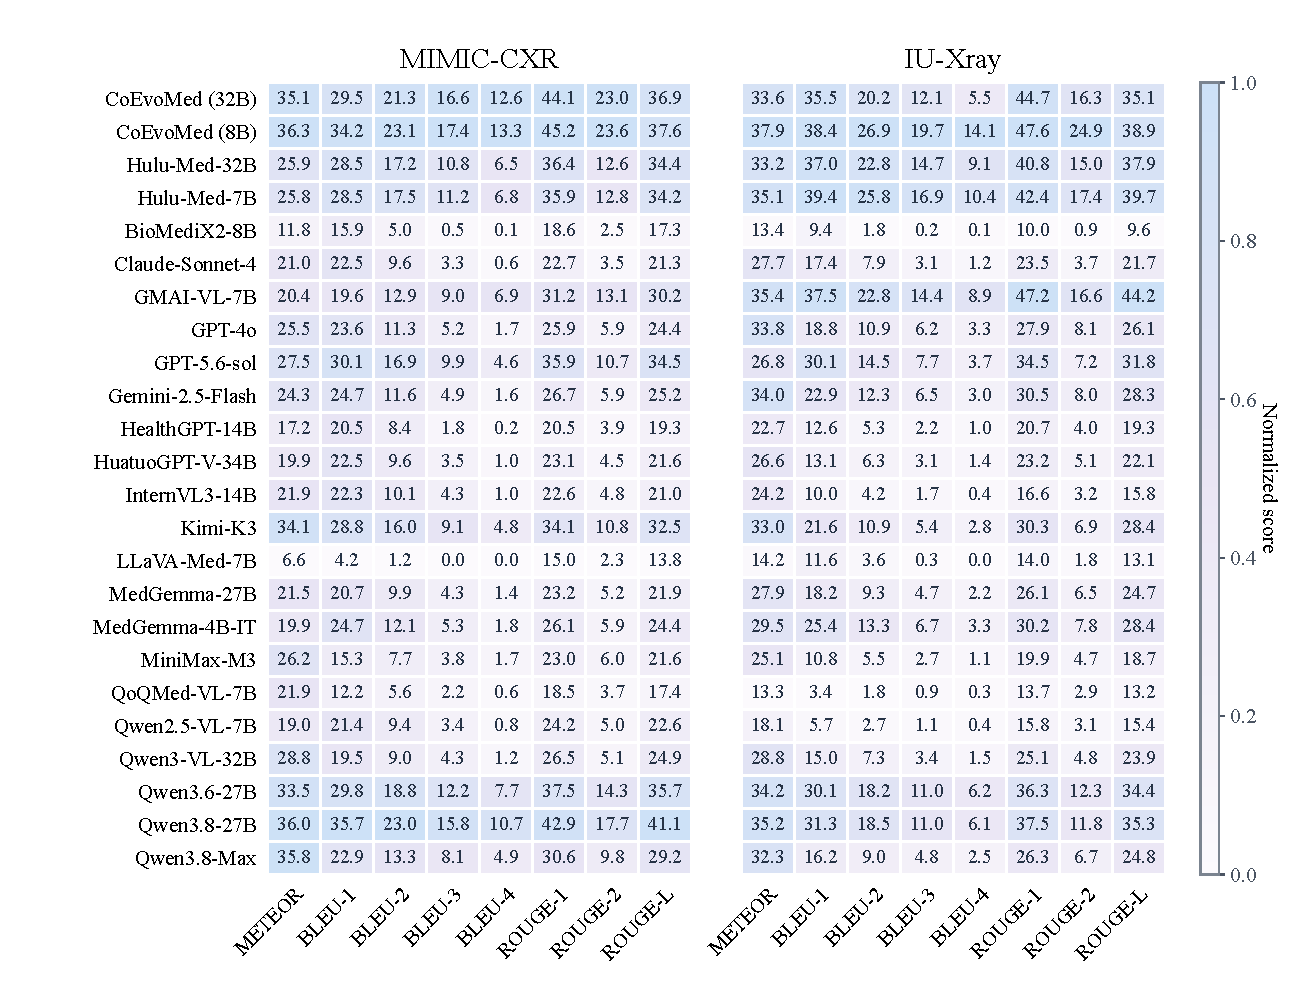
\includegraphics[width=\linewidth]{figures/report_lexical.pdf}
\caption{Supplementary lexical metrics for MIMIC-CXR and IU-Xray report generation. Cells show scores on a 0--100 scale, rounded to one decimal; colors are min--max normalized within each metric and dataset. Higher is better. ``--'' marks unavailable values and is not treated as zero.}
\label{fig:report_lexical}
\end{figure}

\paragraph{Volumetric benchmark results.}

Figure~\ref{fig:3d_appendix_profiles} reports recognition, open-ended question answering, and report generation results. CoEvoMed leads all five M3D-VQA categories, with 80.11\% overall accuracy (11,048/13,791) and 83.06\% macro-averaged accuracy across categories; Med3DVLM-7B (Med3DVLM-Qwen-2.5-7B)~\citep{xin2025med3dvlm} reaches 79.18\% overall accuracy. These results support CoEvoMed's applicability across complementary volumetric medical tasks.

\begin{figure}[!htbp]
\centering
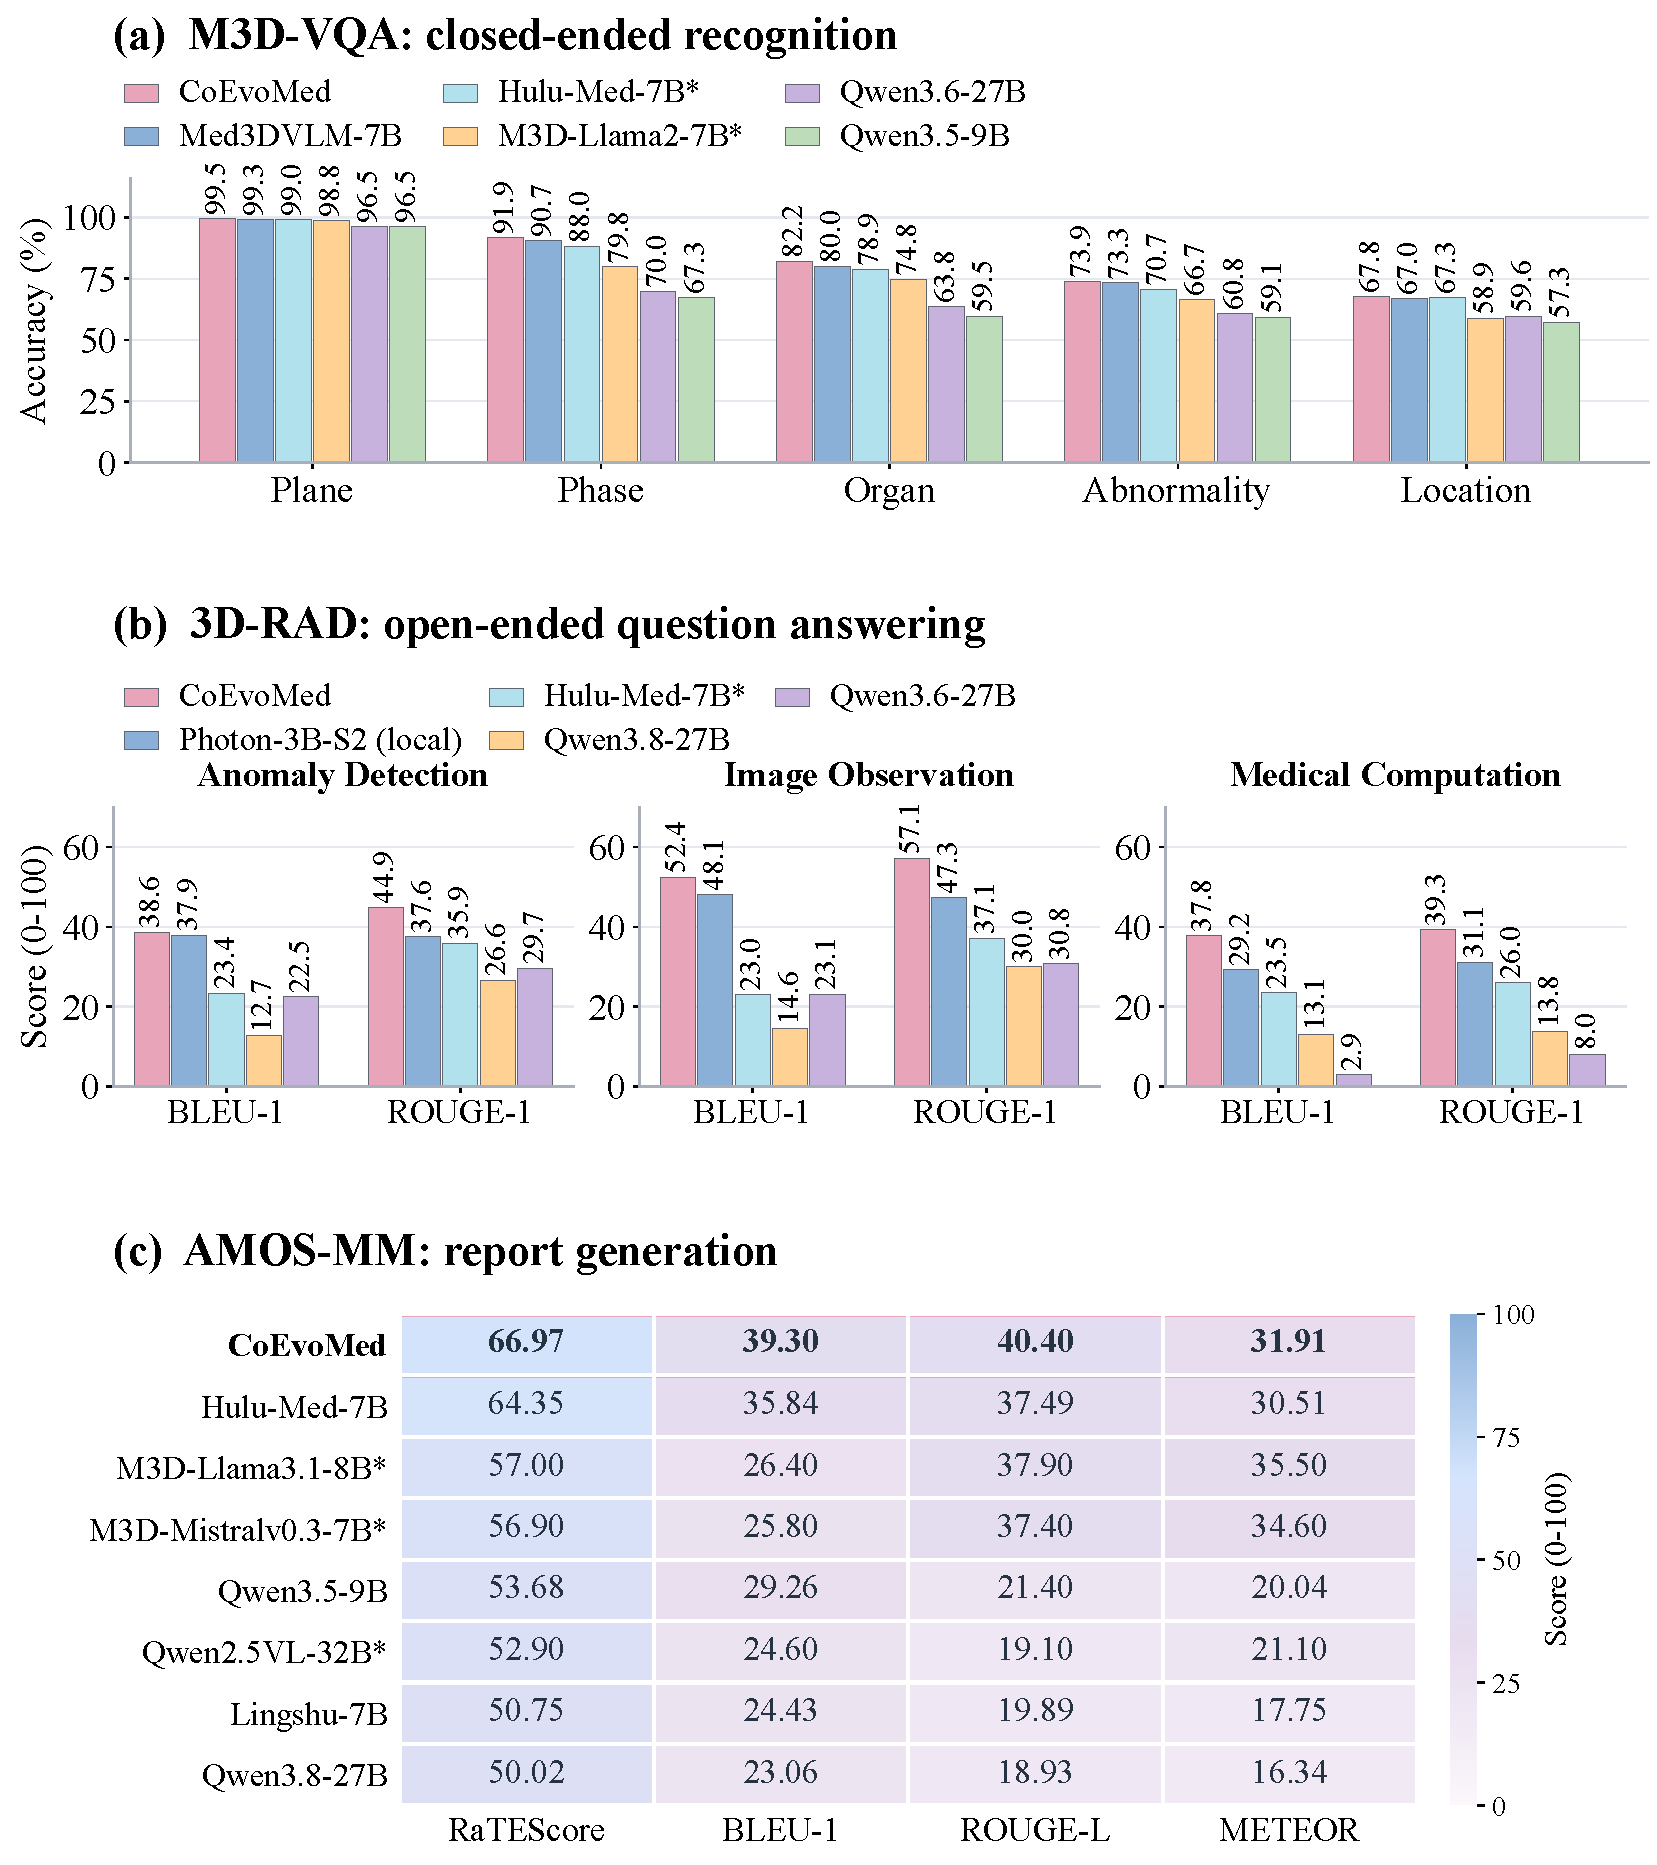
\includegraphics[width=\linewidth]{figures/three_d_appendix_profiles.pdf}
\caption{Detailed 3D benchmark profiles. (a) M3D-VQA closed-ended accuracy across five categories. (b) 3D-RAD open-ended BLEU-1 and ROUGE-1 across three tasks; Photon uses its local S2 evaluation. (c) AMOS-MM report generation metrics, with raw values and a fixed 0--100 color scale. Each panel includes CoEvoMed and the highest-ranked available baselines: five by mean category accuracy in (a), four by mean task ROUGE-1 in (b), and seven by RaTEScore in (c). All scores are scaled to 100. Asterisks mark results from \citet{jiang2025hulumed}.}
\label{fig:3d_appendix_profiles}
\end{figure}


\subsection{Construction of support evidence and validation sets}

The support pool $\mathcal S$ provides source evidence for supervision construction. Validation sets $\mathcal V=\{\mathcal V_t\}_{t\in\mathcal T}$ organized by task assess learner capabilities and guide adaptation through capability estimates, error semantics, and curriculum returns. External benchmark collections $\mathcal B_{\mathrm{ext}}$ are used to report performance of the final model and intermediate checkpoints. We detail the construction of support evidence and validation sets below.

The task taxonomy $\mathcal T$ defines the units used for validation feedback. Support sources and their roles in supervision construction are detailed below. The evaluation datasets and input processing for 2D and volumetric tasks are described together in Appendix~\ref{app:datasets_2d}. Gemma-3-4B-IT trajectories appear in the main text (Figure~\ref{fig:gemma_trajectory}); InternVL3-9B results appear in Appendix~\ref{app:internvl}. InternVL3-9B uses independently trained models for the two tasks.

\paragraph{2D support sources.}
\label{app:support_2d}
The 2D support pool contains 259,767 source records drawn from 11 datasets, spanning medical publication figures, radiological and pathological images, and associated text and labels. Figure~\ref{fig:support_composition} summarizes the source composition, and Table~\ref{tab:support_links} provides official resource links.

\paragraph{3D support sources.}
\label{app:support_3d}
The 3D support pool contains 215,657 source records drawn from five datasets, comprising 209,329 question--answer pairs and 6,328 reports. It covers anatomical recognition, localization, abnormality characterization, and report generation. The question--answer pairs correspond to 4,228 unique videos, each consisting of 64 ordered slices. Figure~\ref{fig:support_composition} summarizes the source composition, and Table~\ref{tab:support_links} provides official resource links.

\begin{figure}[!htbp]
\centering
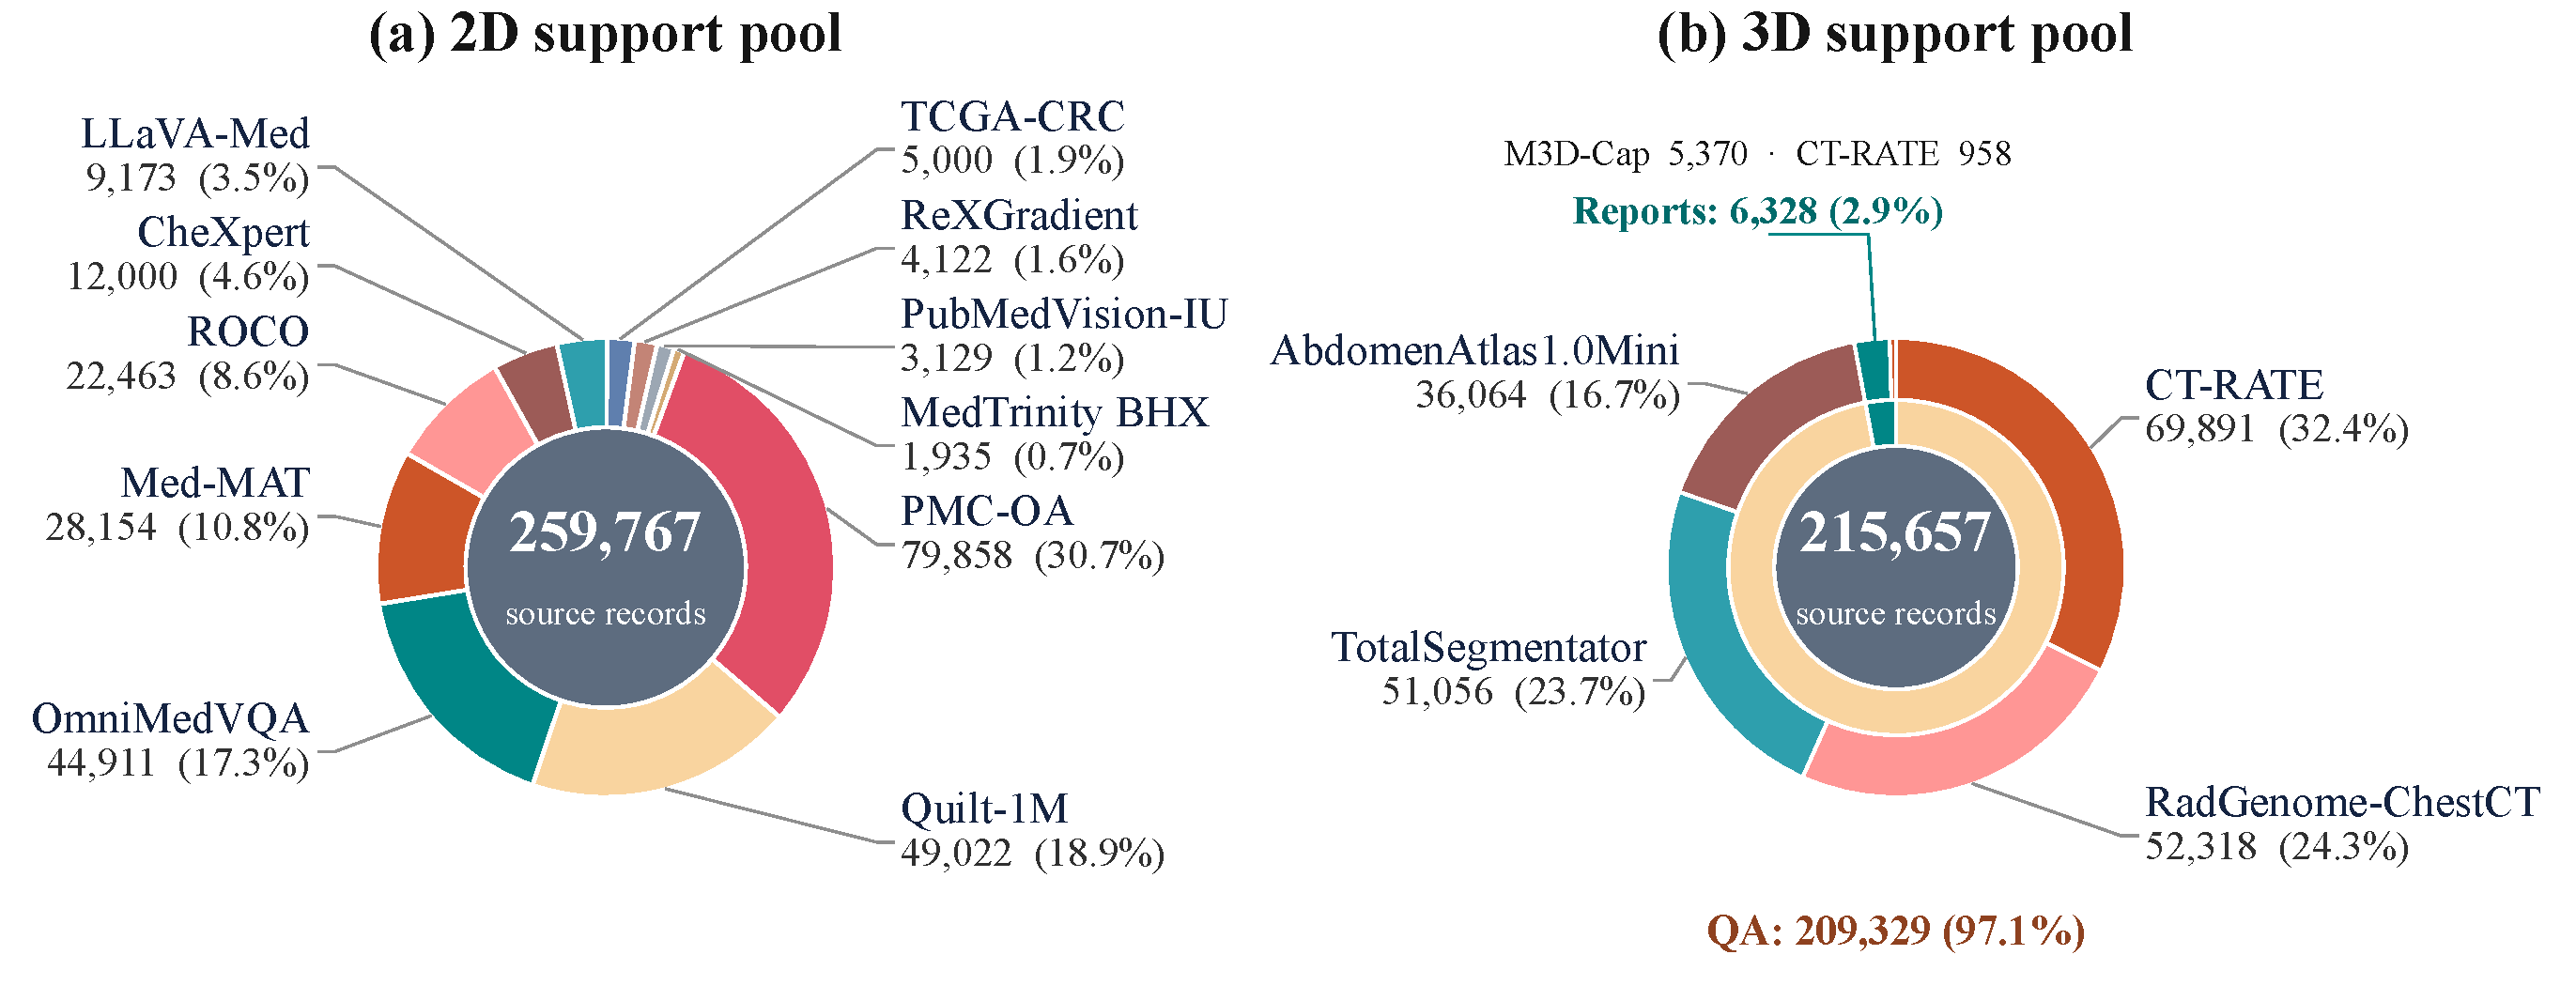
\includegraphics[width=\linewidth]{figures/support_composition.pdf}
\caption{Support-source composition. (a) The 2D support pool contains 259,767 source records. (b) The 3D support pool contains 215,657 source records: the inner ring separates question--answer pairs and reports, and the outer ring identifies their sources. Sector areas and percentages are relative to the total in each panel.}
\label{fig:support_composition}
\end{figure}

\begin{table}[htb]
\centering\small
\caption{Official resources for the support sources. Links for PubMedVision-IU, MedTrinity BHX, and TCGA-CRC lead to their parent datasets.}
\label{tab:support_links}
\setlength{\tabcolsep}{4pt}
\def\UrlFont{\footnotesize\sffamily}
\def\UrlBigBreaks{}
\begin{tabularx}{\linewidth}{@{}L{.28\linewidth}Y@{}}
\toprule
Dataset & Official resource\\
\midrule
\multicolumn{2}{@{}l}{\textit{2D support}}\\
PMC-OA\newline\citep{lin2023pmcclip} & \url{https://weixionglin.github.io/PMC-CLIP/}\\
Quilt-1M\newline\citep{ikezogwo2023quilt} & \url{https://github.com/wisdomikezogwo/quilt1m}\\
OmniMedVQA\newline\citep{hu2024omnimedvqa} & \url{https://github.com/OpenGVLab/Multi-Modality-Arena}\\
Med-MAT\newline\citep{cai2025medmat} & \url{https://github.com/FreedomIntelligence/Med-MAT}\\
ROCO\newline\citep{pelka2018roco} & \url{https://github.com/razorx89/roco-dataset}\\
CheXpert\newline\citep{irvin2019chexpert} & \url{https://aimi.stanford.edu/datasets/chexpert-chest-x-rays}\\
LLaVA-Med\newline\citep{li2023llava} & \url{https://github.com/microsoft/LLaVA-Med}\\
TCGA-CRC\newline\citep{tcga2012colorectal} & \url{https://gdc.cancer.gov/about-data/publications/coadread_2012}\\
ReXGradient\newline\citep{zhang2025rexgradient} & \url{https://huggingface.co/datasets/rajpurkarlab/ReXGradient-160K}\\
PubMedVision-IU subset\newline\citep{chen2024pubmedvision} & \url{https://huggingface.co/datasets/FreedomIntelligence/PubMedVision}\\
MedTrinity BHX\newline\citep{xie2025medtrinity} & \url{https://github.com/UCSC-VLAA/MedTrinity-25M}\\
\midrule
\multicolumn{2}{@{}l}{\textit{3D support}}\\
AbdomenAtlas1.0Mini\newline\citep{li2024abdomenatlas} & \url{https://huggingface.co/datasets/AbdomenAtlas/AbdomenAtlas1.0Mini}\\
CT-RATE\newline\citep{hamamci2026ctrate} & \url{https://huggingface.co/datasets/ibrahimhamamci/CT-RATE}\\
RadGenome-ChestCT\newline\citep{zhang2025radgenome} & \url{https://huggingface.co/datasets/RadGenome/RadGenome-ChestCT}\\
TotalSegmentator\newline\citep{wasserthal2023totalsegmentator} & \url{https://github.com/wasserth/TotalSegmentator}\\
M3D-Cap\newline\citep{bai2024m3d} & \url{https://huggingface.co/datasets/GoodBaiBai88/M3D-Cap}\\
\bottomrule
\end{tabularx}
\end{table}


% Based on the author's updated 数据加工.txt; 500 is a target size, and 359,355 counts facts.
\begin{samepage}
\paragraph{Source evidence normalization and fact extraction.}
\label{app:data_preparation}
Source preparation converts heterogeneous medical image--text records into reusable factual evidence for learner-conditioned supervision construction. Each record retains its visual input, original text, and source association; report instances preserve multiple images from the same study. Native question--answer pairs and classification labels are converted into factual statements through rule-based transformations, reports are organized by Findings and Impression, and facts are extracted from image captions using Qwen3.6-27B. Source records are annotated along four dimensions---task form, visual capability, imaging modality, and anatomical region---to align evidence retrieval with the capability targets specified by the curriculum.

Quality control examines structural completeness, medical relevance, and factual completeness; records without usable facts are excluded from supervision construction. New records are deduplicated by sample identifier, image path, and RGB pixel content, with additional checks for image overlap with the validation collection. The resulting source pool provides 359,355 reusable facts. This count refers to fact entries, distinct from the source record counts in Figure~\ref{fig:support_composition}.

\par
\end{samepage}

\paragraph{Task-based construction of validation sets.}
Validation sets take medical tasks as their organizing units, with stratified selection from existing medical VQA and report data according to task-specific input attributes and output requirements. Question answering tasks are stratified by language, answer type, question form, and content category; multiple-choice tasks additionally account for correct options and question length. Report generation tasks are stratified by input attributes such as image count. Each validation subset targets 500 instances and preserves instance identifiers, images, questions, and original reference annotations. The resulting task-specific collections support ongoing estimation of learner capabilities and learning responses under different task conditions.

\paragraph{Task-based four-dimensional annotation and capability diagnosis.}
Four-dimensional annotation characterizes the task conditions of each validation instance through its capability targets and evidence attributes (Table~\ref{tab:feedback_axes}). Task form and visual capability describe the output structure and principal capability target, while imaging modality and anatomy characterize the underlying medical evidence. Task form is assigned from task requirements and answer format. For visual question answering instances, Qwen3.6-27B supplements the other three dimensions from the image, question, and reference answer, preserving existing modality annotations. Chest X-ray report tasks are labeled as report generation, holistic description, chest X-ray, and chest. Following format and completeness checks, validation performance is aggregated by these task attributes to characterize capability profiles across these targets and identify task priorities for subsequent supervision construction and curriculum allocation.

\begin{table}[H]
\centering\small
\caption{Task-based annotation of validation sets. Task form and visual capability describe capability targets; modality and anatomy describe evidence attributes. Together, they organize task-level capability diagnosis and curriculum adaptation. The visual capability dimension comprises nine categories.}
\label{tab:feedback_axes}
\setlength{\tabcolsep}{4pt}
\renewcommand{\arraystretch}{1.12}
\begin{tabularx}{\linewidth}{@{}lYY@{}}
\toprule
Dimension & Categories or content & Annotation basis\\
\midrule
Task form & Yes/no QA, short open-ended QA, long open-ended QA, multiple choice, report generation & Task requirements and answer format.\\
Visual capability & Modality recognition, organ recognition, localization, spatial relations, abnormality detection, attribute assessment, comparison, holistic description, medical knowledge & The principal capability tested; reports use holistic description.\\
Imaging modality & CT, MRI, X-ray, ultrasound, pathology images, publication figures, etc. & Existing annotations, supplemented by the model when absent.\\
Anatomy or tissue & Chest, abdomen, brain, pelvis, limbs, spine, and specific organs or tissues & Visual and textual evidence; unresolved labels remain unknown / other.\\
\bottomrule
\end{tabularx}
\end{table}

\paragraph{\rev{Agreement with native labels.}}
\rev{The visual capability categories build on the question types of SLAKE~\citep{liu2021slake}, which physicians annotated and which span more modalities and body regions than earlier datasets; VQA-RAD~\citep{lau2018dataset} and M3D-VQA (Figure~\ref{fig:3d_appendix_profiles}a) use similar types. On 200 SLAKE questions, our labels agree with SLAKE's native annotations for 97.5\% of capability categories (Cohen's $\kappa=0.958$, almost perfect agreement under the scale of \citet{landis1977measurement}), 100\% of imaging modalities, and 96.5\% of body regions.}


\subsection{Metrics and statistical reporting}

VQA accuracy is computed using predefined exact or semantic matching criteria. Report evaluation includes BLEU-4, METEOR, and ROUGE-L \citep{papineni2002bleu,banerjee2005meteor,lin2004rouge}. The implemented feedback composite is
$0.5\,\mathrm{ROUGE\mbox{-}L}+0.3\,\mathrm{BLEU\mbox{-}4}+0.2\,\mathrm{METEOR}$.
Feedback scores $U_t^{\mathrm{val}}$ are computed on $\mathcal V_t$, while the controlled comparisons use independent external tests. Figure~\ref{fig:report_results} uses RaTEScore, a separate clinical report metric \citep{zhao2024ratescore}, scaled by 100. RaTEScore does not retrospectively replace feedback scores used for curriculum allocation. Metric implementations and exact/semantic matching choices must be fixed before controlled comparisons. Experiments~1 and~2 report scores and paired contrasts in Tables~\ref{tab:feedback_full} and~\ref{tab:stage_full}.

For longitudinal capability analysis, freeze cell definitions, sample panels within $\mathcal V_t$, decoding settings, and scoring rules in which higher scores indicate better performance before comparison. Compute $\mathcal J_c[M_e]$ on fixed nonempty validation sets, reporting case counts, per-cell changes, and repaired/regressed case transitions. Learning responses are characterized by evaluation metrics aligned with each task's objective. Independent validation feedback at round $e$ guides subsequent curriculum allocation and revision of construction principles. External benchmarks evaluate model performance across rounds and do not inform curriculum decisions. Figure~\ref{fig:trajectory} reports all ten recorded rounds, including later performance declines. Sparse cells are reported as unsupported, not interpreted as evidence of capability change.

\paragraph{Checkpoint selection.}
\label{app:checkpoint_selection}
The CoEvoMed-8B checkpoint is selected according to the overall balance of medical question answering and report generation across training rounds. R7 provides the most balanced overall capability profile among the ten recorded rounds and is used for all six main 2D results. Evaluation using the same checkpoint preserves the joint capability profile of a single learner; individual benchmark peaks occur at R7--R8 in Figure~\ref{fig:trajectory}.

\subsection{InternVL3-9B cross-backbone evaluation}
\label{app:internvl}

Figure~\ref{fig:internvl_trajectory} reports InternVL3-9B trajectories on VQA-RAD and MIMIC-CXR. The two tasks use independently trained models, with full-parameter supervised fine-tuning through LLaMA-Factory~\citep{zheng2024llamafactory}; each round continues from the preceding round's weights. The curves include the baseline and all eight completed training rounds.

VQA-RAD accuracy increases from 56.98\% to 77.38\% at round 8, a gain of 20.40 percentage points, and peaks at 78.71\% at round 6. MIMIC-CXR RaTEScore increases from 50.55 to 63.83, a gain of 13.28 points, with a maximum of 65.34 at round 4. The two trajectories reach their maxima at different stages and retain substantial gains at the final round.

\begin{figure}[H]
\centering
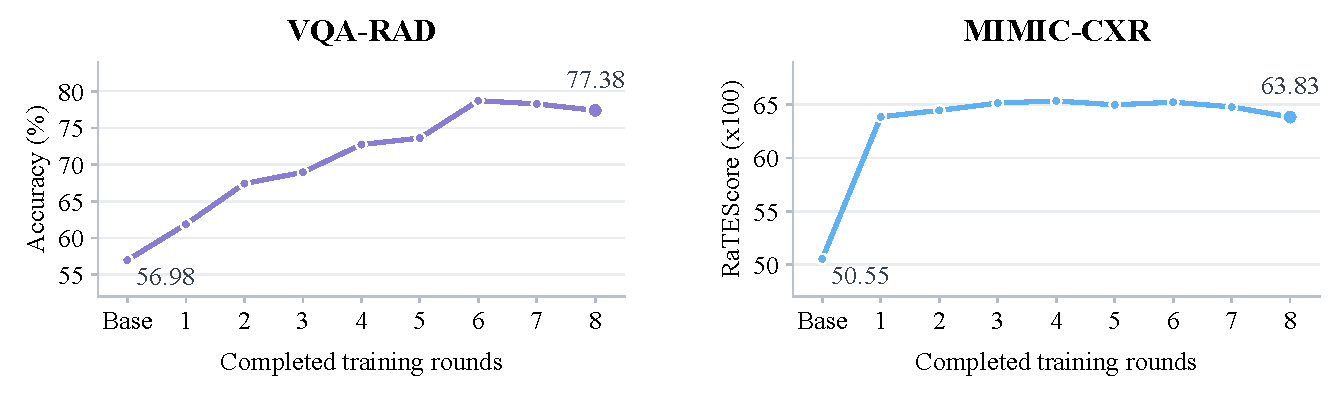
\includegraphics[width=\linewidth]{figures/internvl_trajectory.pdf}
\caption{InternVL3-9B learning trajectories. Left: VQA-RAD accuracy (\%). Right: MIMIC-CXR RaTEScore, scaled by 100. The panels correspond to independently trained task-specific models. Base denotes the initial model; rounds 1--8 denote completed training rounds. Only baseline and final values are annotated.}
\label{fig:internvl_trajectory}
\end{figure}


\subsection{Feedback provenance and independence}

CoEvoMed uses validation sets $\mathcal V$ organized by task and independent of the final evaluation data. Learning responses on these validation sets provide capability estimates and curriculum rewards and guide the revision of construction principles. External benchmark collections $\mathcal B_{\mathrm{ext}}$ are reserved for performance evaluation and do not participate in supervision construction, learner training, or curriculum and principle updates.

\section{Curriculum interventions and component controls}
\label{app:mechanisms}

\subsection{Experiment 1: feedback--learner alignment}
\label{app:feedback_ablation}

Experiment 1 fixes the learner's initial state at R5 and uses historical validation feedback from R2 or R3, or current R5 feedback. Feedback comprises numerical capability statistics describing task-level mastery and learning changes, and summaries of error semantics characterizing unresolved failure modes. Both components are jointly replaced with records from the same source round to guide curriculum allocation and supervision construction, testing alignment between validation-based diagnosis and the current learner state. Table~\ref{tab:feedback_full} extends panel A of Table~\ref{tab:ablations} to six 2D benchmarks under the evaluation settings in Appendix~\ref{app:datasets_2d}. All changes are measured against the same R5 reference scores measured before further training. The condition using current feedback shares its training result with condition D of Experiment 2 and corresponds to round 6 in Figure~\ref{fig:trajectory}.

\begin{table}[H]
\centering\scriptsize
\caption{Full results with the R5 learner fixed and numerical capability statistics and summaries of error semantics jointly replaced by R2, R3, or R5 feedback. VQA reports accuracy (\%); report generation uses RaTEScore ($\times100$). Parentheses give changes from the R5 reference scores measured before further training.}
\label{tab:feedback_full}
\setlength{\tabcolsep}{3pt}
\renewcommand{\arraystretch}{1.18}
\begin{tabularx}{\linewidth}{@{}Yrrrrrr@{}}
\toprule
Condition & VQA-RAD & SLAKE & PMC-VQA & PathVQA & MIMIC-CXR & IU-Xray\\
\midrule
R5 reference & 73.61 & 89.00 & 64.60 & 65.80 & 59.00 & 61.63\\
R2 feedback & 72.51 ($-1.10$) & 83.80 ($-5.20$) & 61.00 ($-3.60$) & 62.70 ($-3.10$) & 59.11 ($+0.11$) & 58.61 ($-3.02$)\\
R3 feedback & 71.84 ($-1.77$) & 83.20 ($-5.80$) & 62.80 ($-1.80$) & 63.40 ($-2.40$) & 58.16 ($-0.84$) & 57.59 ($-4.04$)\\
\rowcolor{mainOurs} \textbf{R5 feedback} & 76.23 ($+2.62$) & 89.69 ($+0.69$) & 65.12 ($+0.52$) & 66.93 ($+1.13$) & 61.77 ($+2.77$) & 62.91 ($+1.28$)\\
\bottomrule
\end{tabularx}
\end{table}

Current R5 feedback outperforms both conditions using historical feedback and the reference scores measured before further training on all six benchmarks. Gains over the reference are 2.62 percentage points on VQA-RAD and 2.77 points on MIMIC-CXR, and 0.69, 0.52, 1.13, and 1.28 points on SLAKE, PMC-VQA, PathVQA, and IU-Xray, respectively. R3 feedback reduces performance on all six benchmarks, whereas R2 feedback yields only a marginal improvement on MIMIC-CXR; their relative ordering varies across tasks. These results support jointly updating numerical and semantic feedback to align subsequent curriculum interventions with the learner's current capabilities and error patterns.

\subsection{Experiment 2: stage-dependent utility of construction principles}
\label{app:stage_transfer}

Experiment 2 applies original and evolved construction principles to learners after two (R2) and five (R5) completed training rounds. Conditions A/B initialize from the R2 checkpoint and C/D from R5, followed by training interventions using their assigned principles. Table~\ref{tab:stage_full} extends panel B of Table~\ref{tab:ablations} in the main text to six benchmarks under the same evaluation settings as Experiment 1. Changes are measured against reference scores measured before further training at the corresponding stage. The R5 reference and condition D correspond to rounds 5 and 6 in Figure~\ref{fig:trajectory}.

\begin{table}[H]
\centering\scriptsize
\caption{Complete Experiment 2 results on six 2D benchmarks. Parentheses give changes from reference scores measured before further training at the corresponding stage.}
\label{tab:stage_full}
\setlength{\tabcolsep}{3pt}
\renewcommand{\arraystretch}{1.18}
\begin{tabularx}{\linewidth}{@{}Yrrrrrr@{}}
\toprule
Condition & VQA-RAD & SLAKE & PMC-VQA & PathVQA & MIMIC-CXR & IU-Xray\\
\midrule
R2 reference & 61.64 & 81.60 & 50.80 & 62.00 & 53.31 & 52.87\\
A: R2 / original & 63.42 ($+1.78$) & 84.20 ($+2.60$) & 54.20 ($+3.40$) & 65.80 ($+3.80$) & 56.35 ($+3.04$) & 56.77 ($+3.90$)\\
B: R2 / evolved & 59.20 ($-2.44$) & 81.00 ($-0.60$) & 48.00 ($-2.80$) & 65.40 ($+3.40$) & 56.47 ($+3.16$) & 56.69 ($+3.82$)\\
\midrule
R5 reference & 73.61 & 89.00 & 64.60 & 65.80 & 59.00 & 61.63\\
C: R5 / original & 67.97 ($-5.64$) & 85.40 ($-3.60$) & 55.00 ($-9.60$) & 63.60 ($-2.20$) & 52.56 ($-6.44$) & 57.52 ($-4.11$)\\
\rowcolor{mainOurs} D: R5 / evolved & 76.23 ($+2.62$) & 89.69 ($+0.69$) & 65.12 ($+0.52$) & 66.93 ($+1.13$) & 61.77 ($+2.77$) & 62.91 ($+1.28$)\\
\bottomrule
\end{tabularx}
\end{table}

All four VQA benchmarks exhibit a reversal in principle ordering: original principles perform better at R2, whereas evolved principles perform better at R5. On VQA-RAD, original principles lead by 4.22 percentage points at R2, while evolved principles lead by 8.26 at R5. The score differences (evolved minus original) on SLAKE, PMC-VQA, and PathVQA change from $-3.20$, $-6.20$, and $-0.40$ to $+4.29$, $+10.12$, and $+3.33$ percentage points, respectively. Both report tasks benefit from either version at R2, with small differences between the two principle versions: evolved principles lead by 0.12 points on MIMIC-CXR, while original principles lead by 0.08 on IU-Xray. At R5, evolved principles lead by 9.21 and 5.39 points, respectively. Condition D improves over the R5 reference on all six benchmarks. These results show that the utility of construction principles varies with learner stage, supporting their continued revision in response to learning.

\subsection{Training on a larger collection of raw data}
\label{app:raw_source}

This comparison examines whether increasing the volume of raw data can account for CoEvoMed's performance gains. Starting from the same Qwen3-VL-8B initialization, Qwen3+Raw trains directly on approximately 700,000 original source examples, exceeding the number of training examples used by CoEvoMed. It retains the original supervision without supervision reconstruction or adaptive curriculum allocation. We evaluate both conditions on the four VQA benchmarks in Appendix~\ref{app:datasets_2d}.

\begin{table}[!htbp]
\centering\small
\caption{Medical VQA accuracy (\%) from a shared Qwen3-VL-8B initialization. Qwen3+Raw uses approximately 700,000 source examples; CoEvoMed uses fewer training examples. The base model is included as a reference.}
\label{tab:raw_source}
\setlength{\tabcolsep}{7pt}
\begin{tabular}{@{}lrrrr@{}}
\toprule
Training condition & PMC-VQA & VQA-RAD & SLAKE & PathVQA\\
\midrule
Qwen3-VL-8B (base) & 54.13 & 56.76 & 64.84 & 42.77\\
Qwen3+Raw & 45.51 & 43.01 & 38.15 & 35.94\\
\rowcolor{mainOurs} CoEvoMed-8B & \textbf{67.95} & \textbf{82.48} & \textbf{91.60} & \textbf{69.40}\\
\bottomrule
\end{tabular}
\end{table}

Despite using less training data, CoEvoMed exceeds Qwen3+Raw by 22.44, 39.47, 53.45, and 33.46 percentage points on PMC-VQA, VQA-RAD, SLAKE, and PathVQA, respectively. Training directly on source data falls below the initial model on all four benchmarks, whereas CoEvoMed improves on each. Thus, a larger collection of raw data does not reproduce CoEvoMed's gains. These results support the effectiveness of supervision construction driven by learning responses and curriculum adaptation in translating source evidence into supervision suited to the learner's evolving needs.

\section{Scope of the formulation}
\label{sec:limitations}

The curriculum construction map is a stochastic, learner-conditioned transformation. Experience generation and allocation shape learning trajectories by influencing capability development through training. Finite validation panels provide partial capability evidence, and covered cells retain their own scoring scales. Independent external tests assess generalization after repeated validation-driven adaptation.

Local interventions establish evidence at the tested learner states and construction versions. Applicability claims are restricted to the evaluated data and backbone-specific settings. Medical benchmark performance and source-grounded verification do not establish clinical safety or patient benefit.

\section{Formal model and notation}
\label{app:formalization}

This appendix formalizes the co-evolution described in Section~\ref{sec:problem}. The learner $M_e$ and the agents' construction principles $\Sigma_e$ are reciprocally dependent components of the complete state $X_e$. The map $\mathfrak C_e$ in Equation~\ref{eq:construction} combines allocation, active principles, and evidence verification to produce supervision for the learner update. Responses obtained after the learner update enter history and inform principle revision; $\Phi(h_e)$ supplies the input to the allocation policy. Fixed $\mathcal J_c$ evaluate successive capabilities to form the trajectory $\Gamma_E=(\widehat{\boldsymbol\kappa}_0,\ldots,\widehat{\boldsymbol\kappa}_E)$ over $E$ rounds. The allocation policy optimizes cumulative validation progress within these coupled dynamics.

\subsection{Capability profile and validation observations}

Equation~\ref{eq:capability_level} defines empirical mastery $\mathcal J_c[M_e]$ through a capability evaluation functional that maps the learner's predictive behavior on a fixed validation set to a scalar capability coordinate. The fixed validation set $\mathcal V_c$ and instance-level evaluation rule $u_c$ determine this functional. Each $\mathcal V_c$ belongs to the validation set $\mathcal V_t$ for its task; example identities, scoring rules, and decoding settings are fixed before comparison. Equation~\ref{eq:capability_change} measures learning progress as the difference in the same functional evaluated on successive learners, equivalently the mean of paired instance-level evaluation changes on the same set. Initial assessment provides mastery levels; missing observations are marked separately.

VQA feedback records repaired and regressed cases. Report feedback tracks score changes and persistent low scores on $\mathcal V_t$; a fixed low-score criterion defines report gaps, rather than one minus a composite score. The feedback summary retains current performance, changes between consecutive rounds, capability gaps, and previous allocations.

Let $o_e$ denote the validation observation at round $e$, including measured performance and error evidence. The observable interaction history is
\[
h_e=(o_0,a_0,r_0,\ldots,a_{e-1},r_{e-1},o_e),
\qquad \mathbf{s}_e=\Phi(h_e).
\]
Here $a_e$ is a curriculum action, $r_e$ is the reward in Equation~\ref{eq:gain}, and $\Phi$ compresses history into the planner's input. Round $e$ uses $\Sigma_e$ to construct supervision and update the learner, then appends $a_e,r_e,o_{e+1}$ to history. Equation~\ref{eq:strategy_evolution} uses the resulting $h_{e+1}$ to revise principles, producing $\Sigma_{e+1}$ for the next round. The curriculum planner acts on the history summary; the transition of the complete system state is defined on $X_e$.

\subsection{Complete state and partially observable dynamics}

For a prescribed rule $\mathscr E$ governing the evolution of construction principles, the finite-horizon process is
\[
\mathcal M_{\mathscr E}=(\mathcal X,\mathcal A_{\mathrm{act}},\mathcal O,P_{\mathscr E},\Omega,R,\rho_0,\gamma,E).
\]
The spaces $\mathcal X$, $\mathcal A_{\mathrm{act}}$, and $\mathcal O$ contain complete system states, admissible curriculum actions, and validation observations, respectively. The kernel $P_{\mathscr E}$ describes state transitions including updates to construction principles, and $\Omega$ describes observations conditional on the complete state. The reward rule $R$ produces the reward in Equation~\ref{eq:gain}; $\rho_0$ is the initial state distribution, $\gamma$ the discount factor, and $E$ the number of decision rounds.

The state $X_e\in\mathcal X$ contains the learner parameters and training state, active construction principles, retained training data, feedback and evolution statistics, scheduling information, and remaining resources. The state retains the information required for subsequent updates under the fixed execution rules.
Equation~\ref{eq:transition} gives the Markov transition used in the main formulation.
Initialization and observations satisfy $X_0\sim\rho_0$ and $o_e\sim\Omega(\cdot\mid X_e)$. Training-induced capability changes occur within the state transition; they do not require a time-varying transition kernel on this complete state. Construction, filtering, learner optimization, and scheduled updates to construction principles all contribute to the transition. One implementation episode corresponds to one decision step, not an entire POMDP trajectory.

\subsection{Training distribution and resource constraints}

The multi-agent roles in Section~\ref{sec:multiagent} realize the stochastic curriculum construction map
\begin{equation}
\mathcal D_e^{\mathrm{syn}}=\mathfrak C_e(\mathcal S,h_e),
\qquad
\mathfrak C_e=\mathfrak C[\mu_{\theta_e},\Sigma_e].
\label{eq:construction}
\end{equation}
The map combines policy-guided allocation, principle-conditioned generation, and evidence-grounded verification. Its accepted supervision enters the training mixture in Equation~\ref{eq:learning_dynamics}. Equation~\ref{eq:supervision_mixture} characterizes the distribution of candidate examples before verification; the round index includes dependence on current history $h_e$ and curriculum action $a_e$.

Let $z=(v,x,y)$ be a constructed example consisting of a visual input, instruction, and target response. Given feedback $\mathbf{s}_e$, the sampled action $a_e\sim\mu_\theta(\cdot\mid \mathbf{s}_e)$ determines quota shares $q_{e,c}$ for constructing candidate examples through the allocation map. The conditional constructor $g_{\Sigma_e}$ specifies generation using the active construction principles and support evidence. Before quality filtering, their joint contribution is
\begin{equation}
p_e(z,c\mid h_e,a_e,\Sigma_e)
=q_{e,c}\,
g_{\Sigma_e}(z\mid c,\mathcal S,h_e,a_e).
\label{eq:factorization}
\end{equation}
Marginalizing over $c$ yields Equation~\ref{eq:supervision_mixture}, with $g_{e,c}(z;\Sigma_e,\mathcal S)=g_{\Sigma_e}(z\mid c,\mathcal S,h_e,a_e)$. The shares $q_{e,c}$ serve as mixture weights for the candidate distributions, sum to one over $\mathcal C$, and obey Equation~\ref{eq:quota}. This factorization describes the marginal distribution of an example drawn according to candidate quotas; generation within a batch may be dependent. Filtering changes accepted examples and their proportions; realized exposure additionally depends on original or replay data and sampling during training. Candidate counts, accepted counts, training tokens, and costs of model calls are recorded separately.

Principles $\Sigma_e$ and shares $\boldsymbol q_e$ control candidate content and cross-capability composition, respectively; filtering and mixing further determine the training distribution. Learner optimization uses the loss over response tokens in Equation~\ref{eq:student}, allocation is learned through PPO, and principle revision compares examples generated from the same medical evidence (Section~\ref{sec:strategy_evolution}). Fixed validation criteria $\mathcal J_c$ record the resulting capability changes, supplying learning responses for subsequent adaptation.

The shorthand objective in Equation~\ref{eq:objective} restricts the search to policies that satisfy the budget constraints. Writing the initialization and transition dependencies explicitly gives
\begin{equation}
\begin{aligned}
\max_{\pi\in\Pi_{\mathrm{adm}}}\quad&
\E_{\rho_0,\pi,P_{\mathscr E},\Omega}
\left[\sum_{e=0}^{E-1}\gamma^e r_e\right]\\
\text{subject to}\quad&
\sum_{e=0}^{E-1}\mathbf k_e\preceq\mathbf B ,
\end{aligned}
\label{eq:objective_full}
\end{equation}
Here $\Pi_{\mathrm{adm}}$ is the class of policies satisfying constraints on curriculum actions and allocation quotas. The vector $\mathbf k_e$ records resource consumption in round $e$, $\mathbf B$ contains the corresponding total budgets, and $\preceq$ imposes each budget componentwise. The expectation includes stochastic curriculum actions, data construction, and learner updates under the fixed execution procedure.

The prescribed rule governing the evolution of construction principles contributes to state transitions and future learning returns; PPO optimizes the allocation policy. The reward equals the validation gain between consecutive models, with equal weight assigned to VQA and report generation. It retains both improvements and regressions. Performance on independent external benchmarks assesses the resulting generalization separately from discounted training return.

\subsection{Cumulative gains and the learning process}
\label{app:cumulative_gains}

Using the fixed task family weights and scoring scales in Equation~\ref{eq:gain}, define
\[
F_e=\frac{1}{2|\mathcal T_{\mathrm V}|}\sum_{t\in\mathcal T_{\mathrm V}}U_t^{\mathrm{val}}(M_e)
+\frac{1}{2|\mathcal T_{\mathrm R}|}\sum_{t\in\mathcal T_{\mathrm R}}U_t^{\mathrm{val}}(M_e).
\]
Then $r_e=F_{e+1}-F_e$. For a fixed horizon $E\geq1$ and $0<\gamma\leq1$, reindexing gives
\begin{equation}
\begin{aligned}
\sum_{e=0}^{E-1}\gamma^e(F_{e+1}-F_e)
&=\sum_{e=1}^{E}\gamma^{e-1}F_e-\sum_{e=0}^{E-1}\gamma^eF_e\\
&=-F_0+(1-\gamma)\sum_{e=1}^{E-1}\gamma^{e-1}F_e+\gamma^{E-1}F_E.
\end{aligned}
\label{eq:trajectory_objective}
\end{equation}
The identity holds for each interaction trajectory; taking expectations yields an equivalent form of Equation~\ref{eq:objective}. A fixed starting learner makes $F_0$ constant. For $\gamma<1$, intermediate and terminal performance receive nonnegative weights; at $\gamma=1$, the intermediate terms cancel. This scalar objective aggregates task performance, while $\Gamma_E$ retains changes in each capability cell.

\clearpage
\section{Qualitative dialogue examples}
\label{app:showcase}

Figures~\ref{fig:showcase_path_pmc}--\ref{fig:showcase_m3d} present CoEvoMed dialogue examples across six 2D and three 3D benchmarks. Each panel pairs the visual input with user queries and model responses. GT denotes the reference answer.

\begin{figure}[H]
\centering
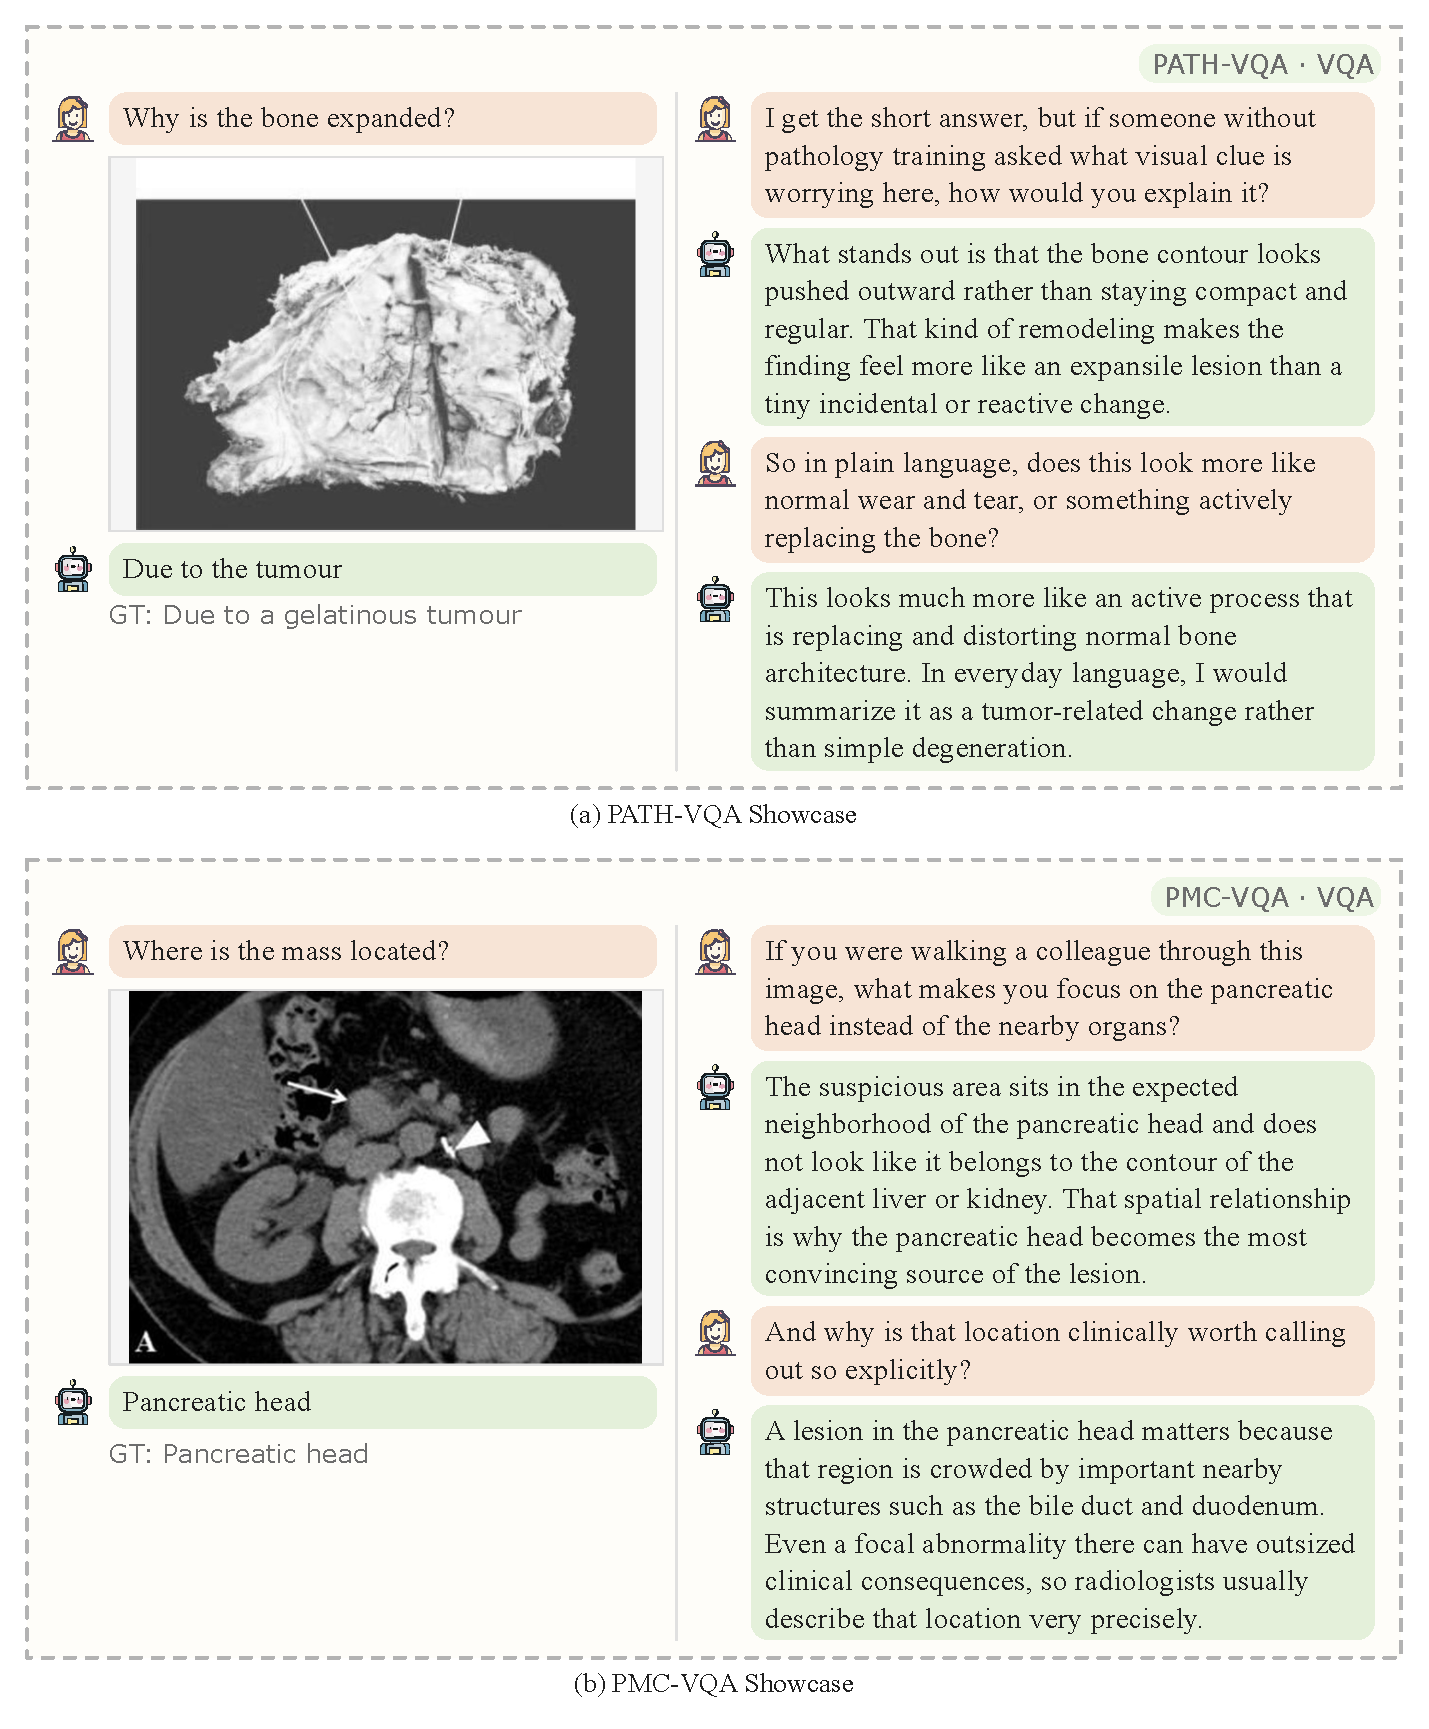
\includegraphics[width=\linewidth]{figures/showcase/medical_vqa_2d.pdf}
\caption{Multi-turn CoEvoMed dialogue examples on PathVQA (top) and PMC-VQA (bottom).}
\label{fig:showcase_path_pmc}
\end{figure}

\clearpage
\begin{figure}[H]
\centering
\includegraphics[page=2,width=\linewidth]{figures/showcase/medical_vqa_2d.pdf}
\caption{Multi-turn CoEvoMed dialogue examples on SLAKE (top) and VQA-RAD (bottom).}
\label{fig:showcase_slake_rad}
\end{figure}

\clearpage
\begin{figure}[H]
\centering
\includegraphics[page=3,width=\linewidth]{figures/showcase/medical_vqa_2d.pdf}
\caption{Multi-turn CoEvoMed dialogue examples for report generation on IU-Xray (top) and MIMIC-CXR (bottom).}
\label{fig:showcase_reports}
\end{figure}

\clearpage
\begin{figure}[H]
\centering
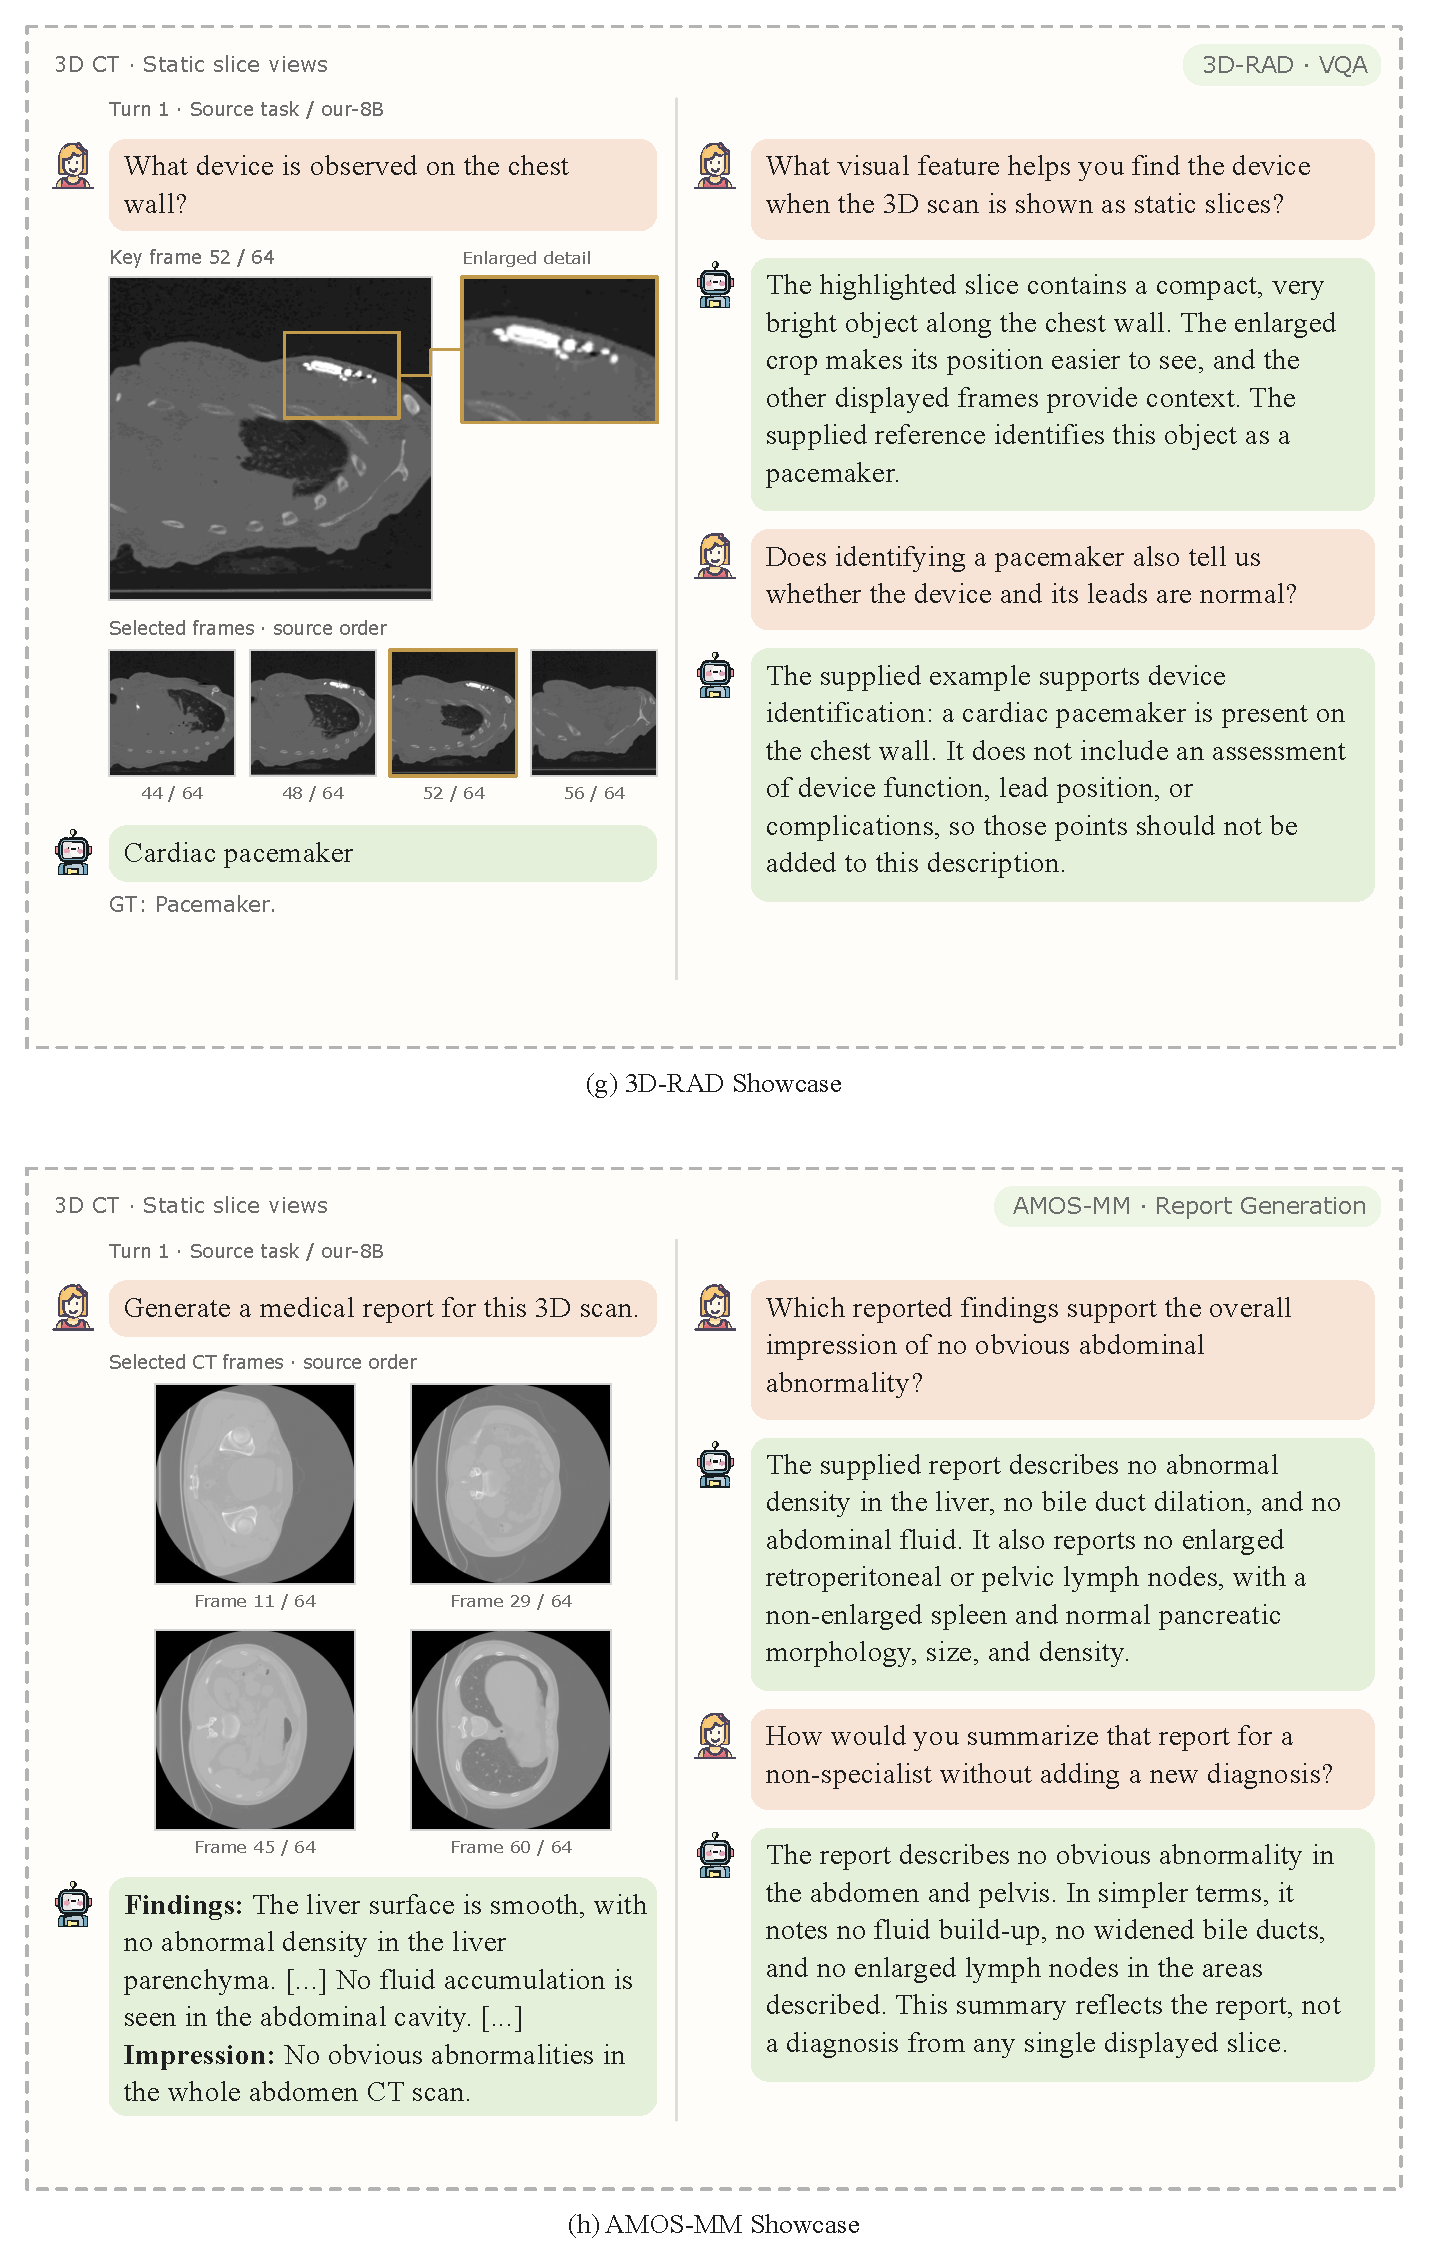
\includegraphics[width=\linewidth,height=0.86\textheight,keepaspectratio]{figures/showcase/medical_vqa_3d_pairs.pdf}
\caption{Multi-turn CoEvoMed dialogue examples on 3D-RAD (top) and AMOS-MM (bottom), with selected CT slices. The AMOS-MM report is excerpted for display; ellipses mark omitted text.}
\label{fig:showcase_rad_amos}
\end{figure}

\clearpage
\begin{figure}[H]
\centering
\includegraphics[page=2,width=\linewidth]{figures/showcase/medical_vqa_3d_pairs.pdf}
\caption{A multi-turn CoEvoMed dialogue example on M3D-VQA, with selected CT slices and an enlarged detail.}
\label{fig:showcase_m3d}
\end{figure}


\end{document}
